\documentclass[12pt,a4paper,parskip=full,abstract=true,BCOR=10mm,twoside,open=right]{scrreprt}
\KOMAoption{bibliography}{totoc}
\KOMAoption{listof}{totoc}

\usepackage[ngerman,english]{babel}
\usepackage[utf8]{inputenc}

%drawings

\usepackage[pdftex]{graphicx}
\graphicspath{{images/}}
\usepackage{tikz}
\usepackage{circuitikz}
\usetikzlibrary{positioning,dsp,chains,fit,scopes,calc,backgrounds,arrows,decorations.pathmorphing,bending,arrows.meta,shapes.misc,matrix,patterns,shadows,circuits.ee.IEC}
\usepackage{tikz-timing}
\makeatletter

\ctikzset{rf/width/.initial=0.75}
\ctikzset{rf/height/.initial=0.75}
\ctikzset{rf/filter/sinewidth/.initial=0.8}
\ctikzset{rf/filter/sineheight/.initial=0.2}
\ctikzset{rf/switch/length/.initial=0.6}


\long\def\pgfrfdeclarenode#1#2#3{
    \pgfdeclareshape{#1}
    {
        \anchor{center}{
            \pgfpointorigin
        }
        \savedanchor\northwest{%
            \pgf@y=\pgfkeysvalueof{/tikz/circuitikz/bipoles/length}
            \pgf@y=\pgfkeysvalueof{/tikz/circuitikz/rf/height}\pgf@y
            \pgf@y=.5\pgf@y
            \pgf@x=\pgfkeysvalueof{/tikz/circuitikz/bipoles/length}
            \pgf@x=.5\pgf@x
            \pgf@x=-\pgfkeysvalueof{/tikz/circuitikz/rf/width}\pgf@x
        }
        \anchor{north}{
            \northwest
            \pgf@x=0pt
        }
        \anchor{south}{
            \northwest
            \pgf@x=0pt
            \pgf@y=-\pgf@y
        }
        \anchor{west}{
            \northwest
            \pgf@y=0pt
        }
        \anchor{east}{
            \northwest
            \pgf@y=0pt
            \pgf@x=-\pgf@x
        }
        \anchor{south west}{
            \northwest
            \pgf@y=-\pgf@y
        }
        \anchor{north east}{
            \northwest
            \pgf@x=-\pgf@x
        }
        \anchor{north west}{
            \northwest
        }
        \anchor{south east}{
            \northwest
            \pgf@x=-\pgf@x
            \pgf@y=-\pgf@y
        }	  
        \anchor{base}{
            \northwest
            \pgf@x=0pt	  	
        }
        \anchorborder{
            \@tempdima=\pgf@x
            \@tempdimb=\pgf@y
            \northwest
            \pgf@xa=-\pgf@x
            \pgf@ya=\pgf@y
            \pgfpointborderrectangle{\pgfpoint{\@tempdima}{\@tempdimb}}{\pgfpoint{\pgf@xa}{\pgf@ya}}
        }
        #3
        \backgroundpath{			
            \pgfsetcolor{\pgfkeysvalueof{/tikz/circuitikz/color}}	

            \northwest
            \pgf@circ@res@up = \pgf@y 
            \pgf@circ@res@down = -\pgf@y
            \pgf@circ@res@right = -\pgf@x
            \pgf@circ@res@left = \pgf@x

            \pgfscope
                \pgfsetcornersarced{\pgfpoint{4pt}{4pt}}
                \pgfpathrectanglecorners{\pgfpoint{\pgf@circ@res@left}{\pgf@circ@res@down}}{\pgfpoint{\pgf@circ@res@right}{\pgf@circ@res@up}}
                \pgfstroke
            \endpgfscope

            #2

        }
    }
}

\long\def\pgfrfdeclaresimplenode#1#2#3#4{
    \pgfdeclareshape{#1}
    {
        \anchor{center}{
            \pgfpointorigin
        }
        \savedanchor\northwest{%
            #2
        }
        \anchor{north}{
            \northwest
            \pgf@x=0pt
        }
        \anchor{south}{
            \northwest
            \pgf@x=0pt
            \pgf@y=-\pgf@y
        }
        \anchor{west}{
            \northwest
            \pgf@y=0pt
        }
        \anchor{east}{
            \northwest
            \pgf@y=0pt
            \pgf@x=-\pgf@x
        }
        \anchor{south west}{
            \northwest
            \pgf@y=-\pgf@y
        }
        \anchor{north east}{
            \northwest
            \pgf@x=-\pgf@x
        }
        \anchor{north west}{
            \northwest
        }
        \anchor{south east}{
            \northwest
            \pgf@x=-\pgf@x
            \pgf@y=-\pgf@y
        }	  
        \anchor{base}{
            \northwest
            \pgf@x=0pt	  	
        }
        #3
        \backgroundpath{			
            #4
        }
    }
}

\long\def\pgfrfdeclaredoublenode#1#2#3{
    \pgfdeclareshape{#1}
    {
        \anchor{center}{
            \pgfpointorigin
        }
        \savedanchor\northwest{%
            \pgf@y=\pgfkeysvalueof{/tikz/circuitikz/bipoles/length}
            \pgf@y=\pgfkeysvalueof{/tikz/circuitikz/rf/height}\pgf@y
            \pgf@y=.5\pgf@y
            \pgf@x=\pgfkeysvalueof{/tikz/circuitikz/bipoles/length}
            \pgf@x=.75\pgf@x
            \pgf@x=-\pgfkeysvalueof{/tikz/circuitikz/rf/width}\pgf@x
        }
        \anchor{north}{
            \northwest
            \pgf@x=0pt
        }
        \anchor{south}{
            \northwest
            \pgf@x=0pt
            \pgf@y=-\pgf@y
        }
        \anchor{west}{
            \northwest
            \pgf@y=0pt
        }
        \anchor{east}{
            \northwest
            \pgf@y=0pt
            \pgf@x=-\pgf@x
        }
        \anchor{south west}{
            \northwest
            \pgf@y=-\pgf@y
        }
        \anchor{north east}{
            \northwest
            \pgf@x=-\pgf@x
        }
        \anchor{north west}{
            \northwest
        }
        \anchor{south east}{
            \northwest
            \pgf@x=-\pgf@x
            \pgf@y=-\pgf@y
        }	  
        \anchor{base}{
            \northwest
            \pgf@x=0pt	  	
        }
        \anchorborder{
            \@tempdima=\pgf@x
            \@tempdimb=\pgf@y
            \northwest
            \pgf@xa=-\pgf@x
            \pgf@ya=\pgf@y
            \pgfpointborderrectangle{\pgfpoint{\@tempdima}{\@tempdimb}}{\pgfpoint{\pgf@xa}{\pgf@ya}}
        }
        #3
        \backgroundpath{			
            \pgfsetcolor{\pgfkeysvalueof{/tikz/circuitikz/color}}	

            \northwest
            \pgf@circ@res@up = \pgf@y 
            \pgf@circ@res@down = -\pgf@y
            \pgf@circ@res@right = -\pgf@x
            \pgf@circ@res@left = \pgf@x

            \pgfscope
                \pgfsetcornersarced{\pgfpoint{4pt}{4pt}}
                \pgfpathrectanglecorners{\pgfpoint{\pgf@circ@res@left}{\pgf@circ@res@down}}{\pgfpoint{\pgf@circ@res@right}{\pgf@circ@res@up}}
                \pgfstroke
            \endpgfscope

            #2

        }
    }
}

\long\def\pgfrfdeclaremonopole#1#2{
    \pgfrfdeclarenode{#1}{#2}{
        \anchor{A}{
            \northwest
            \pgf@y=0pt
        }
    }
}

\long\def\pgfrfdeclarebipole#1#2{
    \pgfrfdeclarenode{#1}{#2}{
        \anchor{A}{
            \northwest
            \pgf@y=0pt
        }
        \anchor{B}{
            \northwest
            \pgf@y=0pt
            \pgf@x=-\pgf@x
        }
    }
}

\long\def\pgfrfdeclarebipoleslash#1#2{
    \pgfrfdeclarebipole{#1}{
        \pgf@circ@res@step = \pgf@circ@res@left
        \pgfmathaddtolength{\pgf@circ@res@step}{4pt - 4pt*cos(-45)}
        \pgfpathmoveto{\pgfpoint{\pgf@circ@res@step}{\pgf@circ@res@step}}
        \pgfpathlineto{\pgfpoint{-\pgf@circ@res@step}{-\pgf@circ@res@step}}
        \pgfusepath{draw}
        #2
    }
}

\long\def\pgfrfdeclaretripole#1#2{
    \pgfrfdeclarenode{#1}{#2}{
        \anchor{A1}{
            \northwest
            \pgf@y=0pt
        }
        \anchor{B1}{
            \northwest
            \pgf@y=0.5\pgf@y
            \pgf@x=-\pgf@x
        }
        \anchor{B2}{
            \northwest
            \pgf@y=-0.5\pgf@y
            \pgf@x=-\pgf@x
        }
    }
}

\long\def\pgfrfdeclarequadpole#1#2{
    \pgfrfdeclarenode{#1}{#2}{
        \anchor{A1}{
            \northwest
            \pgf@y=0.5\pgf@y
        }
        \anchor{A2}{
            \northwest
            \pgf@y=-0.5\pgf@y
        }
        \anchor{B1}{
            \northwest
            \pgf@y=0.5\pgf@y
            \pgf@x=-\pgf@x
        }
        \anchor{B2}{
            \northwest
            \pgf@y=-0.5\pgf@y
            \pgf@x=-\pgf@x
        }
    }
}

\pgfrfdeclarebipole{attenuator}{
    \pgfscope             
        \pgftransformscale{.5}
        \pgfnode{resistorshape}{center}{}{pgf@att}{\pgfusepath{stroke}}
    \endpgfscope
    \pgfpathmoveto{\pgfpoint{\pgf@circ@res@left}{0}}
    \pgfpathlineto{\pgfpointanchor{pgf@att}{b}}
    \pgfpathmoveto{\pgfpoint{\pgf@circ@res@right}{0}}
    \pgfpathlineto{\pgfpointanchor{pgf@att}{a}}
    \pgfusepath{draw}

}

\pgfrfdeclarebipole{vattenuator}{
    \pgfscope             
        \pgftransformscale{.5}
        \pgfnode{resistorshape}{center}{}{pgf@att}{\pgfusepath{stroke}}
    \endpgfscope
    \pgfpathmoveto{\pgfpoint{\pgf@circ@res@left}{0}}
    \pgfpathlineto{\pgfpointanchor{pgf@att}{b}}
    \pgfpathmoveto{\pgfpoint{\pgf@circ@res@right}{0}}
    \pgfpathlineto{\pgfpointanchor{pgf@att}{a}}
    \pgfusepath{draw}
    \pgfpathmoveto{\pgfpoint{0.5\pgf@circ@res@left}{0.7\pgf@circ@res@down}}
    \pgfpathlineto{\pgfpoint{0.5\pgf@circ@res@right}{0.7\pgf@circ@res@up}}
    \pgfsetarrowsend{stealth}
    \pgfusepath{draw}
}

\def\pgfrffiltersinewave{
        \pgfpathmoveto{\pgfpoint{\pgf@xb}{\pgf@yb}}
        \pgfpathsine{\pgfpoint{\pgf@xa}{\pgf@ya}}
        \pgfpathcosine{\pgfpoint{\pgf@xa}{-\pgf@ya}}
        \pgfpathsine{\pgfpoint{\pgf@xa}{-\pgf@ya}}
        \pgfpathcosine{\pgfpoint{\pgf@xa}{\pgf@ya}}
        \advance \pgf@yb by \pgf@circ@res@step
}

\long\def\pgfrfdeclarefilter#1#2{
    \pgfrfdeclarebipole{#1}{
        \pgfscope
            \pgf@yb = 0.5\pgf@circ@res@up
            \pgf@circ@res@step = -0.5\pgf@circ@res@up
            
            \pgf@xa = \ctikzvalof{rf/filter/sinewidth}\pgf@circ@res@right
            \divide \pgf@xa by 2
            \pgf@ya = \ctikzvalof{rf/filter/sineheight}\pgf@circ@res@up
            \pgf@xb = \ctikzvalof{rf/filter/sinewidth}\pgf@circ@res@left

            \pgfrffiltersinewave
            \pgfrffiltersinewave
            \pgfrffiltersinewave
            \pgfstroke
        \endpgfscope
        #2
    }
}

\def\pgfrfstrikewave#1{
    \pgf@ya = 0.5\pgf@circ@res@up
    \pgf@yb = #1\pgf@ya
    \advance \pgf@ya by -\pgf@yb
    \advance \pgf@ya by -2pt
    \pgfpathmoveto{\pgfpoint{-2pt}{\pgf@ya}}
    \advance \pgf@ya by 4pt
    \pgfpathlineto{\pgfpoint{2pt}{\pgf@ya}}
}

\pgfrfdeclarefilter{lowpass}{
    \pgfrfstrikewave{0}
    \pgfrfstrikewave{1}
    \pgfusepath{draw}
}

\pgfrfdeclarefilter{highpass}{
    \pgfrfstrikewave{1}
    \pgfrfstrikewave{2}
    \pgfusepath{draw}
}

\pgfrfdeclarefilter{bandpass}{
    \pgfrfstrikewave{0}
    \pgfrfstrikewave{2}
    \pgfusepath{draw}
}

\pgfrfdeclarefilter{allpass}{
}

\pgfrfdeclaretripole{altswitch}{
    \pgf@xa = \ctikzvalof{rf/switch/length}\pgf@circ@res@left
    \pgfpathmoveto{\pgfpoint{\pgf@circ@res@left}{0}}
    \pgfpathlineto{\pgfpoint{\pgf@xa}{0}}
    \pgfpathlineto{\pgfpoint{-\pgf@xa}{-0.5\pgf@circ@res@up}}
    \pgfpathlineto{\pgfpoint{\pgf@circ@res@right}{-0.5\pgf@circ@res@up}}
    \pgfpathmoveto{\pgfpoint{\pgf@circ@res@right}{0.5\pgf@circ@res@up}}
    \pgfpathlineto{\pgfpoint{-\pgf@xa}{0.5\pgf@circ@res@up}}
    \pgfusepath{draw}
    \pgfpathcircle{\pgfpoint{-\ctikzvalof{rf/switch/length}\pgf@circ@res@left}{-0.5\pgf@circ@res@up}}{1.5pt}
    \pgfusepath{draw,fill}
    \pgfsetfillcolor{white}
    \pgfpathcircle{\pgfpoint{-\ctikzvalof{rf/switch/length}\pgf@circ@res@left}{0.5\pgf@circ@res@up}}{1.5pt}
    \pgfusepath{draw,fill}
    \pgfpathmoveto{\pgfpoint{0}{0.25\pgf@circ@res@down}}
    \pgfmathsetmacro{\tikz@start@angle@temp}{(atan2(0.5*\the\pgf@circ@res@up,2*\ctikzvalof{rf/switch/length}*\the\pgf@circ@res@right))}
    \pgfpatharc{-\tikz@start@angle@temp}{+\tikz@start@angle@temp}{\ctikzvalof{rf/switch/length}\pgf@circ@res@right}
    \pgfsetarrowsend{stealth}
    \pgfusepath{draw}
}

\pgfrfdeclarequadpole{chswitch}{
    \pgf@xa = \ctikzvalof{rf/switch/length}\pgf@circ@res@left
    \pgfpathmoveto{\pgfpoint{\pgf@circ@res@left}{0.5\pgf@circ@res@up}}
    \pgfpathlineto{\pgfpoint{\pgf@circ@res@right}{0.5\pgf@circ@res@up}}
    \pgfpathmoveto{\pgfpoint{\pgf@circ@res@left}{0.5\pgf@circ@res@down}}
    \pgfpathlineto{\pgfpoint{\pgf@circ@res@right}{0.5\pgf@circ@res@down}}
    \pgfusepath{draw}
    \pgfpathmoveto{\pgfpoint{\ctikzvalof{rf/switch/length}\pgf@circ@res@left}{0.5\pgf@circ@res@up}}{1.5pt}
    \pgfpathlineto{\pgfpoint{\ctikzvalof{rf/switch/length}\pgf@circ@res@right}{0.5\pgf@circ@res@down}}{1.5pt}
    \pgfpathmoveto{\pgfpoint{\ctikzvalof{rf/switch/length}\pgf@circ@res@right}{0.5\pgf@circ@res@up}}{1.5pt}
    \pgfpathlineto{\pgfpoint{\ctikzvalof{rf/switch/length}\pgf@circ@res@left}{0.5\pgf@circ@res@down}}{1.5pt}
    \pgfsetdash{{3pt}{2pt}}{0pt}
    \pgfusepath{draw}
    \pgfsetfillcolor{white}
    \pgfsetdash{}{0pt}
    \pgfpathcircle{\pgfpoint{\ctikzvalof{rf/switch/length}\pgf@circ@res@left}{0.5\pgf@circ@res@up}}{1.5pt}
    \pgfpathcircle{\pgfpoint{\ctikzvalof{rf/switch/length}\pgf@circ@res@left}{0.5\pgf@circ@res@down}}{1.5pt}
    \pgfpathcircle{\pgfpoint{\ctikzvalof{rf/switch/length}\pgf@circ@res@right}{0.5\pgf@circ@res@up}}{1.5pt}
    \pgfpathcircle{\pgfpoint{\ctikzvalof{rf/switch/length}\pgf@circ@res@right}{0.5\pgf@circ@res@down}}{1.5pt}
    \pgfusepath{draw,fill}
}

\pgfrfdeclarebipoleslash{adc}{
    \pgfscope
        \pgftransformshift{\pgfpoint{0.5\pgf@circ@res@left}{0.5\pgf@circ@res@up}}
        \pgftext{A}
    \endpgfscope
    \pgfscope
        \pgftransformshift{\pgfpoint{0.5\pgf@circ@res@right}{0.5\pgf@circ@res@down}}
        \pgftext{D}
    \endpgfscope
}

\pgfrfdeclarebipoleslash{dac}{
    \pgfscope
        \pgftransformshift{\pgfpoint{0.5\pgf@circ@res@left}{0.5\pgf@circ@res@up}}
        \pgftext{D}
    \endpgfscope
    \pgfscope
        \pgftransformshift{\pgfpoint{0.5\pgf@circ@res@right}{0.5\pgf@circ@res@down}}
        \pgftext{A}
    \endpgfscope
}

\pgfrfdeclarebipole{amp}{
    \pgfscope             
        \pgftransformscale{.5}
        \pgfnode{buffer}{center}{}{pgf@amp}{\pgfusepath{stroke}}
    \endpgfscope
    \pgfpathmoveto{\pgfpoint{\pgf@circ@res@left}{0}}
    \pgfpathlineto{\pgfpointanchor{pgf@amp}{in}}
    \pgfpathmoveto{\pgfpoint{\pgf@circ@res@right}{0}}
    \pgfpathlineto{\pgfpointanchor{pgf@amp}{out}}
    \pgfusepath{draw}
}

\pgfrfdeclaresimplenode{mixer}
{
    \pgf@y=\pgfkeysvalueof{/tikz/circuitikz/bipoles/length}
    \pgf@y=\pgfkeysvalueof{/tikz/circuitikz/tripoles/mixer/height}\pgf@y
    \pgf@y=.4\pgf@y
    \pgf@y=.5\pgf@y
    \pgf@x=\pgfkeysvalueof{/tikz/circuitikz/bipoles/length}
    \pgf@x=.5\pgf@x
    \pgf@x=.4\pgf@x
    \pgf@x=-\pgfkeysvalueof{/tikz/circuitikz/tripoles/mixer/width}\pgf@x
}
{
    \anchorborder{
        \@tempdima=\pgf@x
        \@tempdimb=\pgf@y
        \northwest
        \pgf@xa=-\pgf@x
        \pgf@ya=\pgf@y
        \pgfpointborderellipse{\pgfpoint{\@tempdima}{\@tempdimb}}{\pgfpoint{\pgf@xa}{\pgf@ya}}
    }
}
{
    \northwest
    \pgf@circ@res@up = \pgf@y 
    \pgf@circ@res@down = -\pgf@y
    \pgf@circ@res@right = -\pgf@x
    \pgf@circ@res@left = \pgf@x
    \pgfscope
        \pgfsetlinewidth{\pgfkeysvalueof{/tikz/circuitikz/bipoles/thickness}\pgflinewidth}
        \pgfpathcircle{\pgfpoint{0}{0}}{\pgf@circ@res@up}
        \pgfusepath{draw}
    \endpgfscope
    \pgfmathsetlength{\pgf@circ@res@step}{\the\pgf@circ@res@right*cos(45)}
    \pgfpathmoveto{\pgfpoint{\pgf@circ@res@step}{\pgf@circ@res@step}}
    \pgfpathlineto{\pgfpoint{-\pgf@circ@res@step}{-\pgf@circ@res@step}}
    \pgfpathmoveto{\pgfpoint{-\pgf@circ@res@step}{\pgf@circ@res@step}}
    \pgfpathlineto{\pgfpoint{\pgf@circ@res@step}{-\pgf@circ@res@step}}
    \pgfusepath{draw}
}


\pgfrfdeclarenode{iqmix}{
    \pgfscope             
        \pgftransformshift{\pgfpoint{0.5\pgf@circ@res@right}{0.5\pgf@circ@res@up}}
        \pgftransformrotate{180}
        \pgftransformscale{.2}
        \pgfnode{mixer}{center}{}{pgf@mixi}{\pgfusepath{stroke}}
    \endpgfscope
    \pgfscope             
        \pgftransformshift{\pgfpoint{0}{0.5\pgf@circ@res@down}}
        \pgftransformrotate{180}
        \pgftransformscale{.2}
        \pgfnode{mixer}{center}{}{pgf@mixq}{\pgfusepath{stroke}}
    \endpgfscope
    \pgfscope             
        \pgftransformscale{.35}
        \pgfnode{rectangle}{center}{$90\degree$}{pgf@phase}{\pgfusepath{stroke}}
    \endpgfscope
    \pgfpathmoveto{\pgfpoint{\pgf@circ@res@left}{0pt}}
    \pgfpathlineto{\pgfpoint{0.6\pgf@circ@res@left}{0pt}}
    \pgfpathlineto{\pgfpoint{0.6\pgf@circ@res@left}{0.5\pgf@circ@res@up}}
    \pgfpathlineto{\pgfpointanchor{pgf@mixi}{out}}
    \pgfpathmoveto{\pgfpoint{0.6\pgf@circ@res@left}{0pt}}
    \pgfpathlineto{\pgfpoint{0.6\pgf@circ@res@left}{0.5\pgf@circ@res@down}}
    \pgfpathlineto{\pgfpointanchor{pgf@mixq}{out}}
    \pgfpathmoveto{\pgfpointanchor{pgf@mixi}{in}}
    \pgfpathlineto{\pgfpoint{\pgf@circ@res@right}{0.5\pgf@circ@res@up}}
    \pgfpathmoveto{\pgfpointanchor{pgf@mixq}{in}}
    \pgfpathlineto{\pgfpoint{\pgf@circ@res@right}{0.5\pgf@circ@res@down}}
    \pgfpathmoveto{\pgfpoint{0pt}{\pgf@circ@res@up}}
    \pgfpathlineto{\pgfpointanchor{pgf@phase}{north}}
    \pgfpathmoveto{\pgfpointanchor{pgf@phase}{south}}
    \pgfpathlineto{\pgfpointanchor{pgf@mixq}{in 2}}
    \pgfpathmoveto{\pgfpoint{0pt}{0.8\pgf@circ@res@up}}
    \pgfpathlineto{\pgfpoint{0.5\pgf@circ@res@right}{0.8\pgf@circ@res@up}}
    \pgfpathlineto{\pgfpointanchor{pgf@mixi}{in 2}}
    \pgfusepath{draw}
    \pgfpathcircle{\pgfpoint{0pt}{0.8\pgf@circ@res@up}}{1pt}
    \pgfpathcircle{\pgfpoint{0.6\pgf@circ@res@left}{0pt}}{1pt}
    \pgfusepath{fill}

}{
    \anchor{A1}{
        \northwest
        \pgf@y=0pt
    }
    \anchor{B1}{
        \northwest
        \pgf@y=0.5\pgf@y
        \pgf@x=-\pgf@x
    }
    \anchor{B2}{
        \northwest
        \pgf@y=-0.5\pgf@y
        \pgf@x=-\pgf@x
    }
    \anchor{C1}{
        \northwest
        \pgf@x=0pt
    }
}

\pgfrfdeclarenode{iqmixdown}{
    \pgfscope             
        \pgftransformshift{\pgfpoint{0.5\pgf@circ@res@right}{0.5\pgf@circ@res@down}}
        \pgftransformscale{.2}
        \pgfnode{mixer}{center}{}{pgf@mixi}{\pgfusepath{stroke}}
    \endpgfscope
    \pgfscope             
        \pgftransformshift{\pgfpoint{0}{0.5\pgf@circ@res@up}}
        \pgftransformscale{.2}
        \pgfnode{mixer}{center}{}{pgf@mixq}{\pgfusepath{stroke}}
    \endpgfscope
    \pgfscope             
        \pgftransformscale{.35}
        \pgfnode{rectangle}{center}{$90\degree$}{pgf@phase}{\pgfusepath{stroke}}
    \endpgfscope
    \pgfpathmoveto{\pgfpoint{\pgf@circ@res@left}{0pt}}
    \pgfpathlineto{\pgfpoint{0.6\pgf@circ@res@left}{0pt}}
    \pgfpathlineto{\pgfpoint{0.6\pgf@circ@res@left}{0.5\pgf@circ@res@down}}
    \pgfpathlineto{\pgfpointanchor{pgf@mixi}{in}}
    \pgfpathmoveto{\pgfpoint{0.6\pgf@circ@res@left}{0pt}}
    \pgfpathlineto{\pgfpoint{0.6\pgf@circ@res@left}{0.5\pgf@circ@res@up}}
    \pgfpathlineto{\pgfpointanchor{pgf@mixq}{in}}
    \pgfpathmoveto{\pgfpointanchor{pgf@mixi}{out}}
    \pgfpathlineto{\pgfpoint{\pgf@circ@res@right}{0.5\pgf@circ@res@down}}
    \pgfpathmoveto{\pgfpointanchor{pgf@mixq}{out}}
    \pgfpathlineto{\pgfpoint{\pgf@circ@res@right}{0.5\pgf@circ@res@up}}
    \pgfpathmoveto{\pgfpoint{0pt}{\pgf@circ@res@down}}
    \pgfpathlineto{\pgfpointanchor{pgf@phase}{south}}
    \pgfpathmoveto{\pgfpointanchor{pgf@phase}{north}}
    \pgfpathlineto{\pgfpointanchor{pgf@mixq}{in 2}}
    \pgfpathmoveto{\pgfpoint{0pt}{0.8\pgf@circ@res@down}}
    \pgfpathlineto{\pgfpoint{0.5\pgf@circ@res@right}{0.8\pgf@circ@res@down}}
    \pgfpathlineto{\pgfpointanchor{pgf@mixi}{in 2}}
    \pgfusepath{draw}
    \pgfpathcircle{\pgfpoint{0pt}{0.8\pgf@circ@res@down}}{1pt}
    \pgfpathcircle{\pgfpoint{0.6\pgf@circ@res@left}{0pt}}{1pt}
    \pgfusepath{fill}

}{
    \anchor{A1}{
        \northwest
        \pgf@y=0pt
    }
    \anchor{B1}{
        \northwest
        \pgf@y=0.5\pgf@y
        \pgf@x=-\pgf@x
    }
    \anchor{B2}{
        \northwest
        \pgf@y=-0.5\pgf@y
        \pgf@x=-\pgf@x
    }
    \anchor{C1}{
        \northwest
        \pgf@x=0pt
        \pgf@y=-\pgf@y
    }
}

\pgfrfdeclarebipole{pll}{
    \pgftext{PLL}
}

\pgfrfdeclarebipole{dut}{
    \pgftext{DUT}
}

\pgfrfdeclarebipole{vna}{
    \pgftext{VNA}
}

\pgfrfdeclarebipole{empty}{
}

\pgfrfdeclaresimplenode{source}
{
    \pgf@y=\pgfkeysvalueof{/tikz/circuitikz/bipoles/length}
    \pgf@y=\pgfkeysvalueof{/tikz/circuitikz/bipoles/vsource/height}\pgf@y
    \pgf@y=.5\pgf@y
    \pgf@x=\pgfkeysvalueof{/tikz/circuitikz/bipoles/length}
    \pgf@x=.5\pgf@x
    \pgf@x=-\pgfkeysvalueof{/tikz/circuitikz/bipoles/vsource/width}\pgf@x
}
{
    \anchorborder{
        \@tempdima=\pgf@x
        \@tempdimb=\pgf@y
        \northwest
        \pgf@xa=-\pgf@x
        \pgf@ya=\pgf@y
        \pgfpointborderellipse{\pgfpoint{\@tempdima}{\@tempdimb}}{\pgfpoint{\pgf@xa}{\pgf@ya}}
    }
}
{
    \northwest
    \pgf@circ@res@up = \pgf@y 
    \pgf@circ@res@down = -\pgf@y
    \pgf@circ@res@right = -\pgf@x
    \pgf@circ@res@left = \pgf@x
    \pgfscope             
        \pgftransformrotate{90}
        \pgfnode{vsourcesinshape}{center}{}{pgf@att}{\pgfusepath{stroke}}
    \endpgfscope
}

\pgfrfdeclaresimplenode{isolator}
{
    \pgf@y=\pgfkeysvalueof{/tikz/circuitikz/bipoles/length}
    \pgf@y=\pgfkeysvalueof{/tikz/circuitikz/bipoles/vsource/height}\pgf@y
    \pgf@y=.5\pgf@y
    \pgf@x=\pgfkeysvalueof{/tikz/circuitikz/bipoles/length}
    \pgf@x=.5\pgf@x
    \pgf@x=-\pgfkeysvalueof{/tikz/circuitikz/bipoles/vsource/width}\pgf@x
}
{
    \anchorborder{
        \@tempdima=\pgf@x
        \@tempdimb=\pgf@y
        \northwest
        \pgf@xa=-\pgf@x
        \pgf@ya=\pgf@y
        \pgfpointborderellipse{\pgfpoint{\@tempdima}{\@tempdimb}}{\pgfpoint{\pgf@xa}{\pgf@ya}}
    }
}
{
    \northwest
    \pgf@circ@res@up = \pgf@y 
    \pgf@circ@res@down = -\pgf@y
    \pgf@circ@res@right = -\pgf@x
    \pgf@circ@res@left = \pgf@x
    \pgfscope
        \pgfsetlinewidth{\pgfkeysvalueof{/tikz/circuitikz/bipoles/thickness}\pgflinewidth}
        \pgfpathcircle{\pgfpoint{0}{0}}{\pgf@circ@res@up}
        \pgfusepath{draw}
        \pgfsetarrowsend{latex}
        \pgfpathmoveto{\pgfpoint{0.8\pgf@circ@res@left}{0pt}}
        \pgfpathlineto{\pgfpoint{0.8\pgf@circ@res@right}{0pt}}
        \pgfusepath{draw}
    \endpgfscope
}

\pgfrfdeclaresimplenode{vphase}
{
    \pgf@y=\pgfkeysvalueof{/tikz/circuitikz/bipoles/length}
    \pgf@y=\pgfkeysvalueof{/tikz/circuitikz/bipoles/vsource/height}\pgf@y
    \pgf@y=.5\pgf@y
    \pgf@x=\pgfkeysvalueof{/tikz/circuitikz/bipoles/length}
    \pgf@x=.5\pgf@x
    \pgf@x=-\pgfkeysvalueof{/tikz/circuitikz/bipoles/vsource/width}\pgf@x
}
{
    \anchorborder{
        \@tempdima=\pgf@x
        \@tempdimb=\pgf@y
        \northwest
        \pgf@xa=-\pgf@x
        \pgf@ya=\pgf@y
        \pgfpointborderellipse{\pgfpoint{\@tempdima}{\@tempdimb}}{\pgfpoint{\pgf@xa}{\pgf@ya}}
    }
}
{
    \northwest
    \pgf@circ@res@up = \pgf@y 
    \pgf@circ@res@down = -\pgf@y
    \pgf@circ@res@right = -\pgf@x
    \pgf@circ@res@left = \pgf@x
    \pgfscope
        \pgfsetlinewidth{\pgfkeysvalueof{/tikz/circuitikz/bipoles/thickness}\pgflinewidth}
        \pgfpathcircle{\pgfpoint{0}{0}}{\pgf@circ@res@up}
        \pgfusepath{draw}
    \endpgfscope
    \pgfscope
        \pgfsetarrowsend{latex}
        \pgfpathmoveto{\pgfpoint{\pgf@circ@res@right}{\pgf@circ@res@up}}
        \pgfpathlineto{\pgfpoint{\pgf@circ@res@left}{\pgf@circ@res@down}}
        \pgfusepath{draw}
    \endpgfscope
}

\pgfrfdeclaresimplenode{tuner}
{
    \pgf@y=\pgfkeysvalueof{/tikz/circuitikz/bipoles/length}
    \pgf@y=\pgfkeysvalueof{/tikz/circuitikz/bipoles/tgeneric/height}\pgf@y
    \pgf@y=.5\pgf@y
    \pgf@x=\pgfkeysvalueof{/tikz/circuitikz/bipoles/length}
    \pgf@x=.5\pgf@x
    \pgf@x=-\pgfkeysvalueof{/tikz/circuitikz/bipoles/tgeneric/width}\pgf@x
}
{
    \anchorborder{
        \@tempdima=\pgf@x
        \@tempdimb=\pgf@y
        \northwest
        \pgf@xa=-\pgf@x
        \pgf@ya=\pgf@y
        \pgfpointborderrectangle{\pgfpoint{\@tempdima}{\@tempdimb}}{\pgfpoint{\pgf@xa}{\pgf@ya}}
    }
}
{
    \northwest
    \pgf@circ@res@up = \pgf@y 
    \pgf@circ@res@down = -\pgf@y
    \pgf@circ@res@right = -\pgf@x
    \pgf@circ@res@left = \pgf@x
    \pgfscope             
        \pgfnode{tgenericshape}{center}{}{pgf@att}{\pgfusepath{stroke}}
    \endpgfscope
}

\pgfrfdeclaresimplenode{amplifier}
{
    \pgf@y=\pgfkeysvalueof{/tikz/circuitikz/bipoles/length}
    \pgf@y=\pgfkeysvalueof{/tikz/circuitikz/bipoles/buffer/height}\pgf@y
    \pgf@y=.5\pgf@y
    \pgf@y=.6\pgf@y
    \pgf@x=\pgfkeysvalueof{/tikz/circuitikz/bipoles/length}
    \pgf@x=.5\pgf@x
    \pgf@x=.4\pgf@x
    \pgf@x=-\pgfkeysvalueof{/tikz/circuitikz/bipoles/buffer/width}\pgf@x
}
{
    \anchorborder{
        \@tempdima=\pgf@x
        \@tempdimb=\pgf@y
        \northwest
        \pgf@xa=-\pgf@x
        \pgf@ya=\pgf@y
        \pgfpointborderrectangle{\pgfpoint{\@tempdima}{\@tempdimb}}{\pgfpoint{\pgf@xa}{\pgf@ya}}
    }
}
{
    \northwest
    \pgf@circ@res@up = \pgf@y 
    \pgf@circ@res@down = -\pgf@y
    \pgf@circ@res@right = -\pgf@x
    \pgf@circ@res@left = \pgf@x
    \pgfscope
        \pgfsetlinewidth{\pgfkeysvalueof{/tikz/circuitikz/bipoles/thickness}\pgflinewidth}
        \pgfpathmoveto{\pgfpoint{\pgf@circ@res@left}{0pt}}
        \pgfpathlineto{\pgfpoint{\pgf@circ@res@right}{\pgf@circ@res@up}}
        \pgfpathlineto{\pgfpoint{\pgf@circ@res@right}{\pgf@circ@res@down}}
        \pgfpathclose
        \pgfusepath{stroke}
    \endpgfscope
}

\pgfrfdeclaresimplenode{match}
{
    \pgf@y=\pgfkeysvalueof{/tikz/circuitikz/bipoles/length}
    \pgf@y=\pgfkeysvalueof{/tikz/circuitikz/bipoles/resistor/height}\pgf@y
    \pgf@y=.5\pgf@y
    \pgf@x=\pgfkeysvalueof{/tikz/circuitikz/bipoles/length}
    \pgf@x=.5\pgf@x
    \pgf@x=-\pgfkeysvalueof{/tikz/circuitikz/bipoles/resistor/width}\pgf@x
}
{
    \anchorborder{
        \@tempdima=\pgf@x
        \@tempdimb=\pgf@y
        \northwest
        \pgf@xa=-\pgf@x
        \pgf@ya=\pgf@y
        \pgfpointborderrectangle{\pgfpoint{\@tempdima}{\@tempdimb}}{\pgfpoint{\pgf@xa}{\pgf@ya}}
    }
}
{
    \northwest
    \pgf@circ@res@up = \pgf@y 
    \pgf@circ@res@down = -\pgf@y
    \pgf@circ@res@right = -\pgf@x
    \pgf@circ@res@left = \pgf@x
    \pgfscope             
        \pgfnode{resistorshape}{center}{}{pgf@att}{\pgfusepath{stroke}}
    \endpgfscope
}

\pgfrfdeclaresimplenode{vmatch}
{
    \pgf@y=\pgfkeysvalueof{/tikz/circuitikz/bipoles/length}
    \pgf@y=\pgfkeysvalueof{/tikz/circuitikz/bipoles/vresistor/height}\pgf@y
    \pgf@y=.5\pgf@y
    \pgf@x=\pgfkeysvalueof{/tikz/circuitikz/bipoles/length}
    \pgf@x=.5\pgf@x
    \pgf@x=-\pgfkeysvalueof{/tikz/circuitikz/bipoles/vresistor/width}\pgf@x
}
{
    \anchorborder{
        \@tempdima=\pgf@x
        \@tempdimb=\pgf@y
        \northwest
        \pgf@xa=-\pgf@x
        \pgf@ya=\pgf@y
        \pgfpointborderrectangle{\pgfpoint{\@tempdima}{\@tempdimb}}{\pgfpoint{\pgf@xa}{\pgf@ya}}
    }
}
{
    \northwest
    \pgf@circ@res@up = \pgf@y 
    \pgf@circ@res@down = -\pgf@y
    \pgf@circ@res@right = -\pgf@x
    \pgf@circ@res@left = \pgf@x
    \pgfscope             
        \pgfnode{vresistorshape}{center}{}{pgf@att}{\pgfusepath{stroke}}
    \endpgfscope
}

\long\def\pgfrfdeclarecoupler#1#2{
    \pgfrfdeclaredoublenode{#1}{
        \pgfpathmoveto{\pgfpoint{\pgf@circ@res@left}{0pt}}
        \pgfpathlineto{\pgfpoint{\pgf@circ@res@right}{0pt}}
        \pgfusepath{draw}
        \pgf@xa = 0.75\pgf@circ@res@left
        \pgfscope
            \pgfsetlinewidth{1pt}
            \advance \pgf@xa by 4pt
            \pgfpathmoveto{\pgfpoint{\pgf@xa}{0pt}}
            \pgfpathlineto{\pgfpoint{-\pgf@xa}{0pt}}
            \pgfpathmoveto{\pgfpoint{\pgf@xa}{0.15\pgf@circ@res@up}}
            \pgfpathlineto{\pgfpoint{-\pgf@xa}{0.15\pgf@circ@res@up}}
            \pgfusepath{draw}
        \endpgfscope
        \pgfscope
            \pgfsetcornersarced{\pgfpoint{4pt}{4pt}}
            #2
            \pgfusepath{draw}
        \endpgfscope
    }{
        \anchor{A1}{
            \northwest
            \pgf@y=0pt
        }
        \anchor{A2}{
            \northwest
            \pgf@x=0.75\pgf@x
        }
        \anchor{B1}{
            \northwest
            \pgf@x=-\pgf@x
            \pgf@y=0pt
        }
        \anchor{B2}{
            \northwest
            \pgf@x=-0.75\pgf@x
        }
    }
}

\pgfrfdeclarecoupler{dircoupler}{
    \pgfpathmoveto{\pgfpoint{0.75\pgf@circ@res@left}{\pgf@circ@res@up}}
    \pgfpathlineto{\pgfpoint{0.75\pgf@circ@res@left}{0.15\pgf@circ@res@up}}
    \pgfpathlineto{\pgfpoint{0.75\pgf@circ@res@right}{0.15\pgf@circ@res@up}}
    \pgfpathlineto{\pgfpoint{0.75\pgf@circ@res@right}{\pgf@circ@res@up}}
}

\pgfrfdeclarecoupler{dircouplera}{
    \pgfpathmoveto{\pgfpoint{0.75\pgf@circ@res@left}{\pgf@circ@res@up}}
    \pgfpathlineto{\pgfpoint{0.75\pgf@circ@res@left}{0.15\pgf@circ@res@up}}
    \pgfpathlineto{\pgfpoint{0pt}{0.15\pgf@circ@res@up}}
}

\pgfrfdeclarecoupler{dircouplerb}{
    \pgfpathmoveto{\pgfpoint{0.75\pgf@circ@res@left}{0.15\pgf@circ@res@up}}
    \pgfpathlineto{\pgfpoint{0.75\pgf@circ@res@right}{0.15\pgf@circ@res@up}}
    \pgfpathlineto{\pgfpoint{0pt}{0.15\pgf@circ@res@up}}
}

\pgfrfdeclaremonopole{generator}{
    \pgfscope             
        \pgftransformscale{.5}
        \pgftransformrotate{90}
        \pgfnode{vsourcesinshape}{center}{}{pgf@att}{\pgfusepath{stroke}}
    \endpgfscope
}

\pgfrfdeclaremonopole{powermeter}{
    \pgfscope             
        \pgftransformscale{.5}
        \pgftransformrotate{-90}
        \pgfnode{fulldiodeshape}{center}{}{pgf@att}{\pgfusepath{stroke}}
    \endpgfscope
    \pgfpathmoveto{\pgfpoint{0pt}{0.7\pgf@circ@res@up}}
    \pgfpathlineto{\pgfpoint{0pt}{0.7\pgf@circ@res@down}}
    \pgfusepath{draw}
}

\pgfrfdeclaremonopole{spectrum analyzer}{
    \pgfpathmoveto{\pgfpoint{0.7\pgf@circ@res@down}{0.8\pgf@circ@res@left}}
    \pgfpathlineto{\pgfpoint{0.7\pgf@circ@res@down}{0.7\pgf@circ@res@right}}
    \pgfpathmoveto{\pgfpoint{0.8\pgf@circ@res@down}{0.7\pgf@circ@res@left}}
    \pgfpathlineto{\pgfpoint{0.7\pgf@circ@res@up}{0.7\pgf@circ@res@left}}
    \pgfusepath{draw}

    \pgfsetcornersarced{\pgfpoint{2pt}{1pt}}
    \pgfpathmoveto{\pgfpoint{0.7\pgf@circ@res@left}{0.6\pgf@circ@res@down}}
    \pgfpathlineto{\pgfpoint{0.55\pgf@circ@res@left}{0.6\pgf@circ@res@down}}
    \pgfpathlineto{\pgfpoint{0.5\pgf@circ@res@left}{0.4\pgf@circ@res@up}}
    \pgfpathlineto{\pgfpoint{0.45\pgf@circ@res@left}{0.6\pgf@circ@res@down}}
    \pgfpathlineto{\pgfpoint{0.05\pgf@circ@res@left}{0.6\pgf@circ@res@down}}
    \pgfpathlineto{\pgfpoint{0}{0.6\pgf@circ@res@up}}
    \pgfpathlineto{\pgfpoint{0.05\pgf@circ@res@right}{0.6\pgf@circ@res@down}}
    \pgfpathlineto{\pgfpoint{0.45\pgf@circ@res@right}{0.6\pgf@circ@res@down}}
    \pgfpathlineto{\pgfpoint{0.5\pgf@circ@res@right}{0.4\pgf@circ@res@up}}
    \pgfpathlineto{\pgfpoint{0.55\pgf@circ@res@right}{0.6\pgf@circ@res@down}}
    \pgfpathlineto{\pgfpoint{0.7\pgf@circ@res@right}{0.6\pgf@circ@res@down}}
    \pgfusepath{draw}
}

\pgfrfdeclaretripole{splitter}{
    \pgfscope             
        \pgftransformshift{\pgfpoint{0.5\pgf@circ@res@right}{0}}
        \pgftransformscale{.2}
        \pgftransformrotate{-90}
        \pgfnode{resistorshape}{center}{}{pgf@att}{\pgfusepath{stroke}}
    \endpgfscope
    \pgfpathmoveto{\pgfpoint{\pgf@circ@res@left}{0}}
    \pgfpathlineto{\pgfpoint{.5\pgf@circ@res@left}{0}}
    \pgfpathlineto{\pgfpoint{.5\pgf@circ@res@right}{.5\pgf@circ@res@up}}
    \pgfpathlineto{\pgfpoint{\pgf@circ@res@right}{.5\pgf@circ@res@up}}
    \pgfpathmoveto{\pgfpoint{.5\pgf@circ@res@left}{0}}
    \pgfpathlineto{\pgfpoint{.5\pgf@circ@res@right}{.5\pgf@circ@res@down}}
    \pgfpathlineto{\pgfpoint{\pgf@circ@res@right}{.5\pgf@circ@res@down}}
    \pgfpathmoveto{\pgfpointanchor{pgf@att}{east}}
    \pgfpathlineto{\pgfpoint{.5\pgf@circ@res@right}{.5\pgf@circ@res@down}}
    \pgfpathmoveto{\pgfpointanchor{pgf@att}{west}}
    \pgfpathlineto{\pgfpoint{.5\pgf@circ@res@right}{.5\pgf@circ@res@up}}
    \pgfusepath{draw}
}

\pgfrfdeclarebipole{dc block}{
    \pgfscope             
        \pgftransformscale{.5}
        \pgfnode{capacitorshape}{center}{}{pgf@att}{\pgfusepath{stroke}}
    \endpgfscope
    \pgfpathmoveto{\pgfpoint{\pgf@circ@res@left}{0}}
    \pgfpathlineto{\pgfpointanchor{pgf@att}{b}}
    \pgfpathmoveto{\pgfpoint{\pgf@circ@res@right}{0}}
    \pgfpathlineto{\pgfpointanchor{pgf@att}{a}}
    \pgfusepath{draw}

}

\pgfrfdeclaredoublenode{oscilloscope}{
    \pgfscope
        \pgfsetcornersarced{\pgfpoint{2pt}{2pt}}
        \pgfpathrectanglecorners{\pgfpoint{0.9\pgf@circ@res@left}{0.4\pgf@circ@res@down}}{\pgfpoint{0.1\pgf@circ@res@left}{0.75\pgf@circ@res@up}}
        \pgfusepath{draw}
    \endpgfscope
    \foreach \posc/\post/\i in {0.2/0.15/4,0.4/0.35/3,0.6/0.55/2,0.8/0.75/1}{
        \pgfscope
            \pgftransformshift{\pgfpoint{\post\pgf@circ@res@left}{0.6\pgf@circ@res@down}}
            \pgftransformscale{.4}
            \pgftext{\i}
            \pgfusepath{draw}
        \endpgfscope
        \pgfpathcircle{\pgfpoint{\posc\pgf@circ@res@left}{0.8\pgf@circ@res@down}}{1pt}
        \pgfusepath{draw}
    }
    \foreach \x in {0,0.2,0.4}{
        \foreach \y in {0.55,0.25,-0.05,-0.35}{
            \pgfpathrectangle{\pgfpoint{\x\pgf@circ@res@right}{\y\pgf@circ@res@up}}{\pgfpoint{2pt}{2pt}}
        }
    }
    \pgfpathrectangle{\pgfpoint{0.6\pgf@circ@res@right}{0\pgf@circ@res@up}}{\pgfpoint{2pt}{2pt}}
    \pgfpathrectangle{\pgfpoint{0.8\pgf@circ@res@right}{0\pgf@circ@res@up}}{\pgfpoint{2pt}{2pt}}
    \pgfpathcircle{\pgfpoint{0.75\pgf@circ@res@right}{0.45\pgf@circ@res@up}}{0.15\pgf@circ@res@right}
    \pgfpathmoveto{\pgfpoint{0.9\pgf@circ@res@left}{0pt}}
    \pgfpathsine{\pgfpoint{0.2\pgf@circ@res@right}{0.2\pgf@circ@res@up}}
    \pgfpathcosine{\pgfpoint{0.2\pgf@circ@res@right}{-0.2\pgf@circ@res@up}}
    \pgfpathsine{\pgfpoint{0.2\pgf@circ@res@right}{-0.2\pgf@circ@res@up}}
    \pgfpathcosine{\pgfpoint{0.2\pgf@circ@res@right}{0.2\pgf@circ@res@up}}
    \pgfpathmoveto{\pgfpoint{0.9\pgf@circ@res@left}{0.4\pgf@circ@res@up}}
    \pgfpathsine{\pgfpoint{0.1\pgf@circ@res@right}{0.1\pgf@circ@res@up}}
    \pgfpathcosine{\pgfpoint{0.1\pgf@circ@res@right}{-0.1\pgf@circ@res@up}}
    \pgfpathsine{\pgfpoint{0.1\pgf@circ@res@right}{-0.1\pgf@circ@res@up}}
    \pgfpathcosine{\pgfpoint{0.1\pgf@circ@res@right}{0.1\pgf@circ@res@up}}
    \pgfpathsine{\pgfpoint{0.1\pgf@circ@res@right}{0.1\pgf@circ@res@up}}
    \pgfpathcosine{\pgfpoint{0.1\pgf@circ@res@right}{-0.1\pgf@circ@res@up}}
    \pgfpathsine{\pgfpoint{0.1\pgf@circ@res@right}{-0.1\pgf@circ@res@up}}
    \pgfpathcosine{\pgfpoint{0.1\pgf@circ@res@right}{0.1\pgf@circ@res@up}}
    \pgfusepath{draw}

}{
    \anchor{A1}{
        \northwest
        \pgf@y=-0.8\pgf@y
        \pgf@x=0.8\pgf@x
    }
    \anchor{A2}{
        \northwest
        \pgf@y=-0.8\pgf@y
        \pgf@x=0.6\pgf@x
    }
    \anchor{A3}{
        \northwest
        \pgf@y=-0.8\pgf@y
        \pgf@x=0.4\pgf@x
    }
    \anchor{A4}{
        \northwest
        \pgf@y=-0.8\pgf@y
        \pgf@x=0.2\pgf@x
    }
}

\pgfrfdeclaresimplenode{circulator}
{
    \pgf@y=\pgfkeysvalueof{/tikz/circuitikz/bipoles/length}
    \pgf@y=\pgfkeysvalueof{/tikz/circuitikz/tripoles/mixer/height}\pgf@y
    \pgf@y=.5\pgf@y
    \pgf@y=\pgfkeysvalueof{/tikz/circuitikz/tripoles/mixer/margin}\pgf@y
    \pgf@x=\pgfkeysvalueof{/tikz/circuitikz/bipoles/length}
    \pgf@x=.5\pgf@x
    \pgf@x=-\pgfkeysvalueof{/tikz/circuitikz/tripoles/mixer/width}\pgf@x
    \pgf@x=\pgfkeysvalueof{/tikz/circuitikz/tripoles/mixer/margin}\pgf@x
}
{
    \anchor{A}{
        \northwest
        \pgf@y=0pt
    }
    \anchor{B}{
        \northwest
        \pgfpointpolar{45}{\pgf@y}
    }
    \anchor{C}{
        \northwest
        \pgfpointpolar{-45}{\pgf@y}
    }
    \anchorborder{
        \@tempdima=\pgf@x
        \@tempdimb=\pgf@y
        \northwest
        \pgf@xa=-\pgf@x
        \pgf@ya=\pgf@y
        \pgfpointborderellipse{\pgfpoint{\@tempdima}{\@tempdimb}}{\pgfpoint{\pgf@xa}{\pgf@ya}}
    }
}
{
    \northwest
    \pgf@circ@res@up = \pgf@y 
    \pgf@circ@res@down = -\pgf@y
    \pgf@circ@res@right = -\pgf@x
    \pgf@circ@res@left = \pgf@x

    \pgfscope
        \pgfsetlinewidth{\pgfkeysvalueof{/tikz/circuitikz/bipoles/thickness}\pgflinewidth}
        \pgfpathcircle{\pgfpoint{0}{0}}{\pgf@circ@res@up}
        \pgfusepath{draw}
    \endpgfscope
    \pgfscope
        \pgfsetarrows{-{latex[length=5mm]}}
        \pgfpathmoveto{\pgfpoint{-0.65\pgf@circ@res@up}{0}}
        \pgfpatharc{180}{0} {0.65\pgf@circ@res@up}
        \pgfusepath{draw}
    \endpgfscope
}

\pgfdeclareshape{vectorgenerator}
{
    \anchor{center}{
        \pgfpointorigin
    }
    \savedanchor\northwest{%
        \pgf@y=\pgfkeysvalueof{/tikz/circuitikz/bipoles/length}
        \pgf@y=\pgfkeysvalueof{/tikz/circuitikz/rf/height}\pgf@y
        \pgf@y=0.75\pgf@y
        \pgf@x=\pgfkeysvalueof{/tikz/circuitikz/bipoles/length}
        \pgf@x=\pgf@x
        \pgf@x=-\pgfkeysvalueof{/tikz/circuitikz/rf/width}\pgf@x
    }
    \anchor{north}{
        \northwest
        \pgf@x=0pt
    }
    \anchor{south}{
        \northwest
        \pgf@x=0pt
        \pgf@y=-\pgf@y
    }
    \anchor{out}{
        \northwest
        \pgf@y=0.33\pgf@y
    }
    \anchor{in}{
        \northwest
        \pgf@x=-\pgf@x
        \pgf@y=-0.33\pgf@y
    }
    \anchor{west}{
        \northwest
        \pgf@y=0pt
    }
    \anchor{east}{
        \northwest
        \pgf@y=0pt
        \pgf@x=-\pgf@x
    }
    \anchor{south west}{
        \northwest
        \pgf@y=-\pgf@y
    }
    \anchor{north east}{
        \northwest
        \pgf@x=-\pgf@x
    }
    \anchor{north west}{
        \northwest
    }
    \anchor{south east}{
        \northwest
        \pgf@x=-\pgf@x
        \pgf@y=-\pgf@y
    }	  
    \anchor{base}{
        \northwest
        \pgf@x=0pt	  	
    }
    \anchorborder{
        \@tempdima=\pgf@x
        \@tempdimb=\pgf@y
        \northwest
        \pgf@xa=-\pgf@x
        \pgf@ya=\pgf@y
        \pgfpointborderrectangle{\pgfpoint{\@tempdima}{\@tempdimb}}{\pgfpoint{\pgf@xa}{\pgf@ya}}
    }
    \backgroundpath{			
        \pgfsetcolor{\pgfkeysvalueof{/tikz/circuitikz/color}}	

        \northwest
        \pgf@circ@res@up = \pgf@y 
        \pgf@circ@res@down = -\pgf@y
        \pgf@circ@res@right = -\pgf@x
        \pgf@circ@res@left = \pgf@x
        \pgf@circ@res@other = 0.33\pgf@circ@res@up

        \pgfscope
            \pgfsetcornersarced{\pgfpoint{4pt}{4pt}}
            \pgfpathrectanglecorners{\pgfpoint{\pgf@circ@res@left}{\pgf@circ@res@down}}{\pgfpoint{\pgf@circ@res@right}{\pgf@circ@res@up}}
            \pgfstroke
        \endpgfscope
        \pgfscope             
            \pgftransformshift{\pgfpoint{0.66\pgf@circ@res@left}{\pgf@circ@res@other}}
            \pgftransformscale{.4}
            \pgftransformrotate{180}
            \pgfnode{buffer}{center}{}{pgf@amp}{\pgfusepath{stroke}}
        \endpgfscope
        \pgfscope
            \pgftransformshift{\pgfpoint{0}{\pgf@circ@res@other}}
            \pgftransformscale{.5}
            \pgfnode{mixer}{center}{}{pgf@mix}{\pgfusepath{stroke}}
        \endpgfscope
        \pgfscope
            \pgftransformshift{\pgfpoint{0.66\pgf@circ@res@right}{\pgf@circ@res@other}}
            \pgftransformscale{.5}
            \pgftransformrotate{90}
            \pgfnode{vsourcesinshape}{center}{}{pgf@att}{\pgfusepath{stroke}}
        \endpgfscope
        \pgfscope
            \pgfpathmoveto{\pgfpoint{0.77\pgf@circ@res@left}{0.17\pgf@circ@res@down}}
            \pgfpathlineto{\pgfpoint{0.55\pgf@circ@res@left}{0.83\pgf@circ@res@up}}
            \pgfsetarrowsend{stealth}
            \pgfusepath{draw}
        \endpgfscope
        \pgfscope
            \pgfsetlinewidth{\pgfkeysvalueof{/tikz/circuitikz/bipoles/thickness}\pgflinewidth}
            \pgftransformshift{\pgfpoint{0.66\pgf@circ@res@right}{-\pgf@circ@res@other}}
            \pgftransformscale{.5}
            \pgfnode{adc}{center}{}{pgf@dac}{\pgfusepath{stroke}}
        \endpgfscope
        \pgfpathmoveto{\pgfpoint{\pgf@circ@res@left}{\pgf@circ@res@other}}
        \pgfpathlineto{\pgfpointanchor{pgf@amp}{out}}
        \pgfpathmoveto{\pgfpointanchor{pgf@amp}{in}}
        \pgfpathlineto{\pgfpointanchor{pgf@mix}{in}}
        \pgfpathmoveto{\pgfpointanchor{pgf@mix}{out}}
        \pgfpathlineto{\pgfpointanchor{pgf@att}{north}}
        \pgfpathmoveto{\pgfpointanchor{pgf@mix}{in 2}}
        \pgfpathlineto{\pgfpoint{0pt}{-\pgf@circ@res@other}}
        \pgfpathlineto{\pgfpointanchor{pgf@dac}{B}}
        \pgfpathmoveto{\pgfpointanchor{pgf@dac}{A}}
        \pgfpathlineto{\pgfpoint{\pgf@circ@res@right}{-\pgf@circ@res@other}}
        \pgfusepath{draw}
    }
}

\makeatother

\makeatletter
\newcommand\currentcoordinate{\the\tikz@lastxsaved,\the\tikz@lastysaved}
\makeatother

%units

\usepackage[binary-units,retain-explicit-plus]{siunitx}
\DeclareSIUnit \belm {Bm}
\DeclareSIUnit \belfs {BFS}
\DeclareSIUnit \samples {S}
\sisetup{per-mode = symbol}

%plots

\usepackage{pgfplots}
\pgfplotsset{compat=1.12}
\pgfplotsset{every axis/.append style={grid=major,legend style={font=\footnotesize}}}
\usepgfplotslibrary{smithchart}
\usepgfplotslibrary{units}
\usepgfplotslibrary{fillbetween}
\usepgfplotslibrary{statistics}
\pgfplotsset{unit code/.code 2 args={\si{#1#2}}}

\usepgfplotslibrary{external}
\tikzsetexternalprefix{figures/}
\tikzexternalize[mode=list and make]
\tikzexternalwritetomakefile{}
\tikzexternalwritetomakefile{.DELETE_ON_ERROR:}
\tikzexternalwritetomakefile{}

%math

\usepackage[cmex10]{amsmath}
\usepackage{amssymb}
\usepackage{gensymb}

\providecommand{\abs}[1]{\lvert#1\rvert}

%source

\usepackage{listings}
\lstset{language=Matlab,numbers=left,numberstyle=\tiny,stepnumber=5,numbersep=5pt,frame=single,
breaklines=true,postbreak=\raisebox{0ex}[0ex][0ex]{\ensuremath{\color{red}\hookrightarrow\space}},
captionpos=b,escapeinside={(*}{*)},mathescape=true}
\usepackage{letltxmacro}
\newcommand*{\SavedLstInline}{}
\LetLtxMacro\SavedLstInline\lstinline
\DeclareRobustCommand*{\lstinline}{%
  \ifmmode
    \let\SavedBGroup\bgroup
    \def\bgroup{%
      \let\bgroup\SavedBGroup
      \hbox\bgroup
    }%
  \fi
  \SavedLstInline
}

%stuff

\usepackage{url}
\usepackage{tocloft} %table of contents modification
\usepackage{subcaption} %subfigures
\usepackage{placeins} % keep floats in check (=sections where they belong)
\usepackage{booktabs} % nicer tables
\usepackage{cite}

\usepackage{scrlayer-scrpage}
\pagestyle{scrheadings}
\automark[chapter]{chapter}
\automark*[section]{}

\def\device#1{\textit{#1}}
\def\signal#1{{\ttfamily #1}}
\def\module#1{{\ttfamily\bfseries #1}}
\def\clk#1{{\itshape\ttfamily #1}}

\usepackage[colorlinks,hyperindex,plainpages=false,
pdftitle={FPGA-based Load-Pull Measurement System},
pdfauthor={Gernot Vormayr},
pdfsubject={Diploma thesis},
pdfpagelabels %,hidelinks
]{hyperref}

% lots of acronyms
\usepackage[acronym]{glossaries}

\newacronym{fpga}{FPGA}{field programmable gate array}
\newacronym{iq}{IQ}{in-phase/quadrature-phase}
\newacronym[longplural={general-purpose inputs/outputs}]{gpio}{GPIO}{general-purpose input/output}
\newacronym{fir}{FIR}{finite impulse response}
\newacronym{gui}{GUI}{graphical user interface}
\newacronym{dc}{DC}{direct current}
\newacronym{ac}{AC}{alternative current}
\newacronym{ui}{UI}{user interface}
\newacronym{rf}{RF}{radio frequency}
\newacronym{pa}{PA}{power amplifier}
\newacronym{mw}{MW}{microwave}
\newacronym{if}{IF}{intermediate frequency}
\newacronym{ram}{RAM}{random access memory}
\newacronym{sparam}{S-parameter}{scattering parameter}
\newacronym{dut}{DUT}{device under test}
\newacronym{emt}{EMT}{electromechanical tuner}
\newacronym{vna}{VNA}{vector network analyzer}
\newacronym{elp}{ELP}{envelope load-pull}
\newacronym{pc}{PC}{personal computer}
\newacronym{adc}{ADC}{analog-to-digital converter}
\newacronym{dac}{DAC}{digital-to-analog converter}
\newacronym{lo}{LO}{local oscillator}
\newacronym{lvds}{LVDS}{low voltage differential signalling}
\newacronym{fft}{FFT}{fast Fourier transform}
\newacronym{dft}{DFT}{discrete Fourier transform}
\newacronym{lp}{LP}{load-pull}
\newacronym{sma}{SMA}{sub-miniature version A}
\newacronym{sata}{SATA}{serial AT attachment}

\makeglossaries

\usepackage[noabbrev]{cleveref} %needs to be last

\pagenumbering{roman}
\begin{document}
\begin{titlepage}
    \enlargethispage{1cm}
    \centering
    \vspace*{5cm}
    {\Huge \textbf{Diploma thesis}}\\
    \vspace*{1cm}
    {\Large FPGA-based Load-Pull Measurement System}

    \vspace*{2cm}
    {\large Gernot ~\textsc{Vormayr} \\ 0425210 \\ } ~\\

    \vspace*{2cm}
    {\today } ~\\

    \vfill
    {Supervisors} ~\\\vspace*{0.1cm}
    {Ass.Prof. Dipl.-Ing. Dr.techn. \large Holger ~\textsc{Arthaber}} ~\\
    {Univ.Ass. Dipl.-Ing. Dr.techn. \large Thomas ~\textsc{Faseth}}
    \vspace*{2cm}

    \rule{\linewidth}{0.4pt}
    \begin{minipage}[t]{0.55\linewidth}
        \flushleft
        \begin{large}
            EMCE - Institute of Electrodynamics, Microwave and Circuit Engineering
        \end{large}\\
        Vienna University of Technology
    \end{minipage}
    \hfill
    \begin{minipage}[t]{0.27\linewidth}
        \flushright
        Gusshausstrasse 25\\
        1040 Vienna\\
        www.emce.tuwien.ac.at
    \end{minipage}
    \vspace*{-3pt}
    \rule{\linewidth}{0.4pt}
    \clearpage
\end{titlepage}

\begin{abstract}
    %TODO
    \begin{itemize}
        \item RFPA
        \item load-pull
        \item the one in this work
        \item verification
    \end{itemize}
\end{abstract}

\begin{otherlanguage}{ngerman}
\begin{abstract}
    %TODO
    \begin{itemize}
        \item RFPA
        \item load-pull
        \item the one in this work
        \item verification
    \end{itemize}
\end{abstract}
\end{otherlanguage}

\renewcommand{\abstractname}{Acknowledgements}
\begin{abstract}
    %TODO
    TODO
\end{abstract}

\tableofcontents

\chapter{Introduction}
\pagenumbering{arabic}
\label{chap:introduction}

At \gls{rf} and \gls{mw} frequencies, the circuit theory with lumped elements, where
voltage and current do not vary over the physical dimension of the elements, is of limited
value. The wavelength at these frequencies is of the order of the circuit
element dimensions. This means that transmission line theory has to be used instead \cite{pozar_mw_engineering_2011}.
This theory applies circuit theory to infinitesimal small pieces of the lumped elements
and introduces the concept of forward and backward traveling power waves.

For this reason, instead of impedance- and admittance matrices, \glspl{sparam}
are commonly used in \gls{rf} and \gls{mw} circuit engineering to describe
$N$-ports (see \cref{fig:sparam,eq:sparam} for a 2-port). $a_n$ denotes the incident and
$b_n$ the reflected power wave. Complex valued $S_{nn}$ represents the
part of $a_n$ that gets reflected at port $n$, where as $S_{nm}$ is the part of $a_m$ that
is transmitted to $b_n$. A set of \glspl{sparam} is only valid for a specific frequency, a
characteristic impedance $Z_0$, and a well defined reference plane (port 1 and port 2 in \cref{fig:sparam}).

\begin{figure}[htb]
    \centering
    \begin{tikzpicture}
        \matrix (box)
        [matrix of nodes,%
         nodes in empty cells,
         nodes={dspnodeopen},
         column sep=1cm,
         row sep=2cm]
        {
            |[coordinate]| & &[4cm] & |[coordinate]| \\
            |[coordinate]| & & & |[coordinate]| \\
        };
        \draw[-latex] (box-1-1) node[anchor=east] {$a_1$} -- (box-1-2);
        \draw[-latex] (box-1-2) -- node[above] {$S_{21}$} (box-1-3);
        \draw[-latex] (box-1-3) -- (box-1-4) node[anchor=west] {$b_2$};

        \draw[latex-] (box-2-1) node[anchor=east] {$b_1$} -- (box-2-2);
        \draw[latex-] (box-2-2) -- node[above] {$S_{12}$} (box-2-3);
        \draw[latex-] (box-2-3) -- (box-2-4) node[anchor=west] {$a_2$};

        \draw[-latex] (box-1-2) to[bend left=30] node[right] {$S_{11}$} (box-2-2);
        \draw[latex-] (box-1-3) to[bend right=30] node[left] {$S_{22}$} (box-2-3);

        \draw ($(box-1-2) + (0,0.7cm)$) rectangle ($(box-2-3) - (0,0.7cm)$);

        \draw[dashed] (box-1-2) -- ++(0,1.5cm) node[anchor=south] {Port 1};
        \draw[dashed] (box-1-3) -- ++(0,1.5cm) node[anchor=south] {Port 2};

        \draw[dashed] (box-2-2) -- ++(0,-1cm);
        \draw[dashed] (box-2-3) -- ++(0,-1cm);
    \end{tikzpicture}
    \caption{\Glspl{sparam} of a 2-port}
    \label{fig:sparam}
\end{figure}

\begin{equation}
    \label{eq:sparam}
    \begin{pmatrix} b_1 \\ b_2 \end{pmatrix} = \begin{pmatrix} S_{11} & S_{12} \\ S_{21} & S_{22} \end{pmatrix} \begin{pmatrix} a_1 \\ a_2 \end{pmatrix}
\end{equation}

For a 1-port there is only the parameter $S_{11}$, which is equivalent to the reflection
coefficient $\Gamma$ and can be also expressed by the input impedance $Z_{in}$ (see
\cref{eq:s11ref} as shown in \cite{pozar_mw_engineering_2011}). This does not necessarily hold for 2-ports, since for a generic
multi-port configuration, also reflections from the devices connected at the other ports
can be seen.
\begin{equation}
    \label{eq:s11ref} \Gamma = S_{11} = \frac{Z_{in}-Z_0}{Z_{in}+Z_0}
\end{equation}

One way to evaluate the \glspl{sparam} at a specific frequency would be connecting
the reference impedance $Z_0$ to the other ports. To measure e.g. $S_{11}$ a matching impedance, equal to the ports reference impedance, has to
be connected to port 2. According to \cref{eq:s11ref} the reflected wave $a_2$
at port 2 is zero in this case. This means that measurements at port 1 can only see the
reflections caused by $S_{11}$. Consequently $S_{11}$ can now be calculated by measuring the incident
and reflected wave at port 1 (see \cref{eq:s11}) \cite{agilent_an_154}.
\begin{align}
    \label{eq:s11} S_{11} & = \left.\frac{b_1}{a_1} \right\rvert_{a_2 = 0}\\
    \label{eq:s21} S_{21} & = \left.\frac{b_2}{a_1} \right\rvert_{a_2 = 0}
\end{align}
Because of connectors and cabling it is often impossible to connect exact matches. Therefor
\glspl{sparam} are measured by sending a power wave into port 1 of the \gls{dut}, measuring
$a_n$ and $b_n$. After that the measurement is repeated with port 2. With measurements from
both ports and calibration measurements, which are necessary to account for systematic errors in the measurement setup,
it is possible to determine every \gls{sparam}. \Glspl{vna} use this method
and can make automated measurements at various frequencies.

As long as a network behaves linearly, what is typical for small incident signals, the \glspl{sparam}
fully describe this network at a specific frequency. Thus they can also be used
to model amplifiers, as long as they exhibit controlled and linear behaviour. Since
class-A \glspl{pa} are nearly linear, \glspl{sparam} can be used to describe the small
signal behaviour. But those \glspl{pa} exhibit a very low efficiency of around \SI{50}{\percent}.
In modern \gls{rf} and \gls{mw} applications the efficiency is increased with specially designed input and
output matching networks, that improve the performance. This comes at the cost of non-linear
behaviour of the \gls{pa} \cite{ghannouchi_load-pull_2013}.

Because of these non-linearities more complex models and verification systems are
needed. One way to measure the characteristics of a non-linear system is the so called
\gls{lp} technique (see \cref{fig:load_coeff}). This measurement system presents a
controllable load impedance (output tuner) to the \gls{dut}. The fixed input tuner is
needed to match the input of the \gls{dut} to the source. \Gls{lp} can be used for obtaining the
\gls{dut} characteristics, and for verifying an implementation. \Gls{lp} also
allows to test the \gls{dut} under realistic operational conditions.

\begin{figure}[htb]
    \centering
    \begin{tikzpicture}
        \tikzpicturedependsonfile{rfsymbols.tex}
        \draw node[source] (source) {}
              node[tuner,right=of source,label=above:{fixed input tuner}] (ituner) {}
              node[dut,right=of ituner] (dut) {}
              node[tuner,right=2 of dut,label=above:{output tuner}] (otuner) {}
              node[match,right=of otuner,label=above:{$Z_0$}] (match) {}
              node[rground,right=0.3 of match,rotate=90,anchor=center] (ground) {};
        \draw ($(dut)!.5!(otuner)$) node[coordinate] (plane) {};

        \draw (source) -- (ituner) -- (dut) -- (otuner) -- (match) -- (ground);

        \draw [dashed] ($(plane) + (0,2)$) node[anchor=south] {Load Reference Plane} -- ($(plane) - (0,2.5)$);

        \draw [latex-] ($(plane) + (0,1.5)$) -- ++(-0.5,0) node[anchor=east] {$Z_L$};

        \draw [-latex] ($(plane) + (0.25,-1)$) node[anchor=west] {$a_2$}-- ++(-0.5,0);
        \draw [latex-] ($(plane) + (0.25,-1.5)$) node[anchor=west] {$b_2$}-- ++(-0.5,0);
        \draw [latex-] ($(plane) + (0,-2)$) -- ++(-0.5,0) node[anchor=east] {$\Gamma_L$};

    \end{tikzpicture}
    \caption{Load reflection coefficient}
    \label{fig:load_coeff}
\end{figure}

The \cref{eq:gl,eq:zl} show the relations between the load reflection coefficient $\Gamma_L$,
the incident wave $a_2$, the reflected
wave $b_2$, and the load impedance $Z_L$ at port 2 of \cref{fig:sparam,fig:load_coeff}. $Z_0$
is the characteristic impedance of the system \cite{hashmi_highly_2011}.
\begin{align}
    \label{eq:gl} \Gamma_L & = \frac{a_2}{b_2} \\
    \label{eq:zl} \Gamma_L & = \frac{Z_L-Z_0}{Z_L+Z_0}
\end{align}
The output tuner in \cref{fig:load_coeff} synthesizes an appropriate $\Gamma_L$
either by varying the phase and magnitude of the reflected wave $a_2$ or by varying
the load impedance $Z_L$. This means, that it is possible to build a \gls{lp}
setup by either using a passive tuner, or feeding a modified wave back to the
\gls{dut}.

There are various types of \gls{lp} measurement setups, which have different
characteristics. One important feature of a \gls{lp} setup is the repeatability of reflection
coefficients. The repeatability is needed to ensure accurate application
specific device models. Another important factor is the tuning range, which
depicts the maximal achievable range of the reflection coefficient $\abs{\Gamma_L}$
(e.g. \cref{fig:range_passive}). Usually passive \gls{lp}
systems have a more limited tuning range than active ones, but provide a
better repeatability \cite{ghannouchi_load-pull_2013}. Tuner speed and tuner
resolution is an additional trade off. High resolution is needed since \glspl{pa} are often
highly sensitive to impedance variations. However a high resolution incurs
a slow tuner speed. An exemplary resolution can be seen in \cref{fig:generic_emt}.
Power handling capability is another extremely important factor. The \gls{lp}
setup has to be capable to sustain the power presented to the tuner without
damage. Which \gls{lp} setup to choose for a specific \gls{dut} depends on
these requirements.

\begin{figure}[htb]
    \begin{subfigure}[b]{.5\linewidth}
        \centering
        \begin{tikzpicture}
            \begin{smithchart}[width=.9\linewidth]
                \addplot[blue,is smithchart cs,mark=o,only marks] file {testdata/generic_emt.data};
            \end{smithchart}
        \end{tikzpicture}
        \caption{\Glsentryshort{emt}}
        \label{fig:generic_emt}
    \end{subfigure}%
    \begin{subfigure}[b]{.5\linewidth}
        \centering
        \begin{tikzpicture}
            \begin{smithchart}[width=.9\linewidth]
                \filldraw[draw=blue,fill=blue,fill opacity=0.2] (cartesian cs:0,0) let \p1 = (cartesian cs:0.75,0) in circle ({\x1});
            \end{smithchart}
        \end{tikzpicture}
        \caption{Passive \gls{lp} system}
        \label{fig:range_passive}
    \end{subfigure}
    \caption{Generic representation of achievable tuning range/points passive \gls{lp}}
\end{figure}

Passive \gls{lp} systems are based on the block diagram in \cref{fig:load_coeff}. Depending on
the desired measurements, additional circuit elements like directional couplers,
power meters, and oscilloscopes are needed. For higher power measurements additional
amplifiers, and attenuators to reduce the output power to acceptable levels might also
be needed. These additional components, the cabling, and connectors add additional loss
on the reflection path, leading to achievable reflection levels $\abs{\Gamma_L} < 1$ with
a maximum usually around 0.75 \cite{de_groote_introduction_2008} (see \cref{fig:range_passive}).

Typically used tuners, consist of a transmission line and a probe that introduces a mismatch
by adding a parallel susceptance. Varying the position of the probe along the transmission
line changes the phase of the impedance mismatch and the distance the magnitude \cite{hashmi_highly_2011}.
Automated positioning can be achieved by adding motors. These tuners are called \glspl{emt}.
Those have to be calibrated before use and achieve reflection levels like shown in
\cref{fig:generic_emt} with up to 10000 points \cite{ghannouchi_load-pull_2013}.

If higher $\abs{\Gamma_L}$-levels  are needed (even levels $> 1$), active \gls{lp} setups
have to be used. There are two categories: closed- and open loop.

\begin{figure}[htb]
    \centering
    \begin{tikzpicture}
        \tikzpicturedependsonfile{rfsymbols.tex}
        \draw node[dut] (dut) {}
              node[circulator,right=2 of dut] (circ) {}
              node[vmatch,right=of circ,label=above:{Attenuator},yshift=1cm] (att) {}
              node[vphase,right=1.5 of att,label=above:{Phase shift}] (phase) {}
              node[amplifier,right=of circ,label=above:{Amplifier},yshift=-1cm] (amp) {};

        \draw ($(dut)!.5!(circ)$) node[coordinate] (plane) {};

        \draw (dut) -- (circ.A);
        \draw (circ.B) -- ($(circ.B |- att)!.5!(att)$) node[coordinate] (upper) {} -- (att) -- (phase) -- ++(1,0) |- (amp) -- ($(circ.C |- amp)!.5!(amp)$) node[coordinate] (lower) {} -- (circ.C);

        \draw [-latex] ($(circ.B) + (-0.2,0.2)$) -- node[sloped,above] {$b_2$} ($(upper) + (-0.2,0.2)$);
        \draw [latex-] ($(circ.C) + (-0.2,-0.2)$) -- node[sloped,below] {$a_2$} ($(lower) + (-0.2,-0.2)$);

        \draw [dashed] ($(plane) + (0,2)$) node[anchor=south] {Load Reference Plane} -- ($(plane) - (0,2.5)$);

        \draw [latex-] ($(plane) + (0,1.5)$) -- ++(-0.5,0) node[anchor=east] {$Z_L$};

        \draw [-latex] ($(plane) + (0.25,-1)$) node[anchor=west] {$a_2$}-- ++(-0.5,0);
        \draw [latex-] ($(plane) + (0.25,-1.5)$) node[anchor=west] {$b_2$}-- ++(-0.5,0);
        \draw [latex-] ($(plane) + (0,-2)$) -- ++(-0.5,0) node[anchor=east] {$\Gamma_L$};
    \end{tikzpicture}
    \caption{Active closed loop \gls{lp} block diagram}
    \label{fig:active_closed_loop}
\end{figure}

Active closed loop \gls{lp} setups generate a modified reflected wave $a_2$ by
modifying the phase and magnitude of $b_2$ and feeding it back to the \gls{dut}.
The functional block diagram, which can be seen in \Cref{fig:active_closed_loop},
is an example of such an active closed loop \gls{lp} setup. With the circulator
the power wave $b_2$ is fed to a variable attenuator, a phase shifter and an
amplifier. These elements enable modifying the phase and the magnitude of $b_2$,
which is again fed back to the \gls{dut} with the circulator. Because of limited
isolation provided by real world circulators this system will oscillate if the loop gain
exceeds the isolation \cite{ghannouchi_load-pull_2013}. This can be circumvented with
an isolator after the amplifier. Another way to improve the stability of the system
is to introduce a bandpass filter into the loop.

\begin{figure}[htb]
    \centering
    \begin{tikzpicture}
        \tikzpicturedependsonfile{rfsymbols.tex}
        \draw node[dut] (dut) {}
              node[isolator,right=2 of dut,rotate=180,anchor=east] (iso) {}
              node[amplifier,right=of iso.west,label=above:Amplifier] (amp) {}
              node[vphase,right=of amp,label=below:{Phase Shift}] (shift) {}
              node[vmatch,right=of shift,label=above:{Attenuator}] (att) {}
              node[source,right=of att,label=below:{Phase Locked Source}] (source) {};

        \draw ($(dut)!.5!(iso)$) node[coordinate] (plane) {};

        \draw (dut) -- (iso) -- (amp) -- (shift) -- (att) -- (source);
        \draw [latex-] ($(iso.west) + (0.2,-0.2)$) -- node[below] {$a_2$} ($(amp.west) + (-0.2,-0.2)$);

        \draw [dashed] ($(plane) + (0,2)$) node[anchor=south] {Load Reference Plane} -- ($(plane) - (0,2.5)$);

        \draw [latex-] ($(plane) + (0,1.5)$) -- ++(-0.5,0) node[anchor=east] {$Z_L$};

        \draw [-latex] ($(plane) + (0.25,-1)$) node[anchor=west] {$a_2$}-- ++(-0.5,0);
        \draw [latex-] ($(plane) + (0.25,-1.5)$) node[anchor=west] {$b_2$}-- ++(-0.5,0);
        \draw [latex-] ($(plane) + (0,-2)$) -- ++(-0.5,0) node[anchor=east] {$\Gamma_L$};
    \end{tikzpicture}
    \caption{Active open loop \gls{lp} block diagram}
    \label{fig:active_open_loop}
\end{figure}

Active open loop \gls{lp} setups work by generating a phase coherent wave with
an external signal generator (see \cref{fig:active_open_loop}). The open loop
approach has the advantage, that it can't oscillate, since there is no closed loop.
It works by generating a signal with a source, that is locked to the generator driving the
source port of the \gls{dut}. Phase and magnitude can be adjusted with the attenuator and
phase shifter. A disadvantage of the open loop system is that the generated waves $a_2$ are
not derived from $b_2$. This implies that the reflection coefficient $\Gamma_L$ not only
depends on the phase shifter and attenuator settings, but also on the \gls{dut} itself.
Therefore, an iterative approach is needed to be able to achieve a specific $\Gamma_L$ \cite{muller_comparison_1994}.

Keeping in mind above discussions, in the course of the presented thesis the following chapters introduce an active closed loop \gls{lp} system, which
is built with a digital attenuator, phase shifter, and loop filter implemented
in a \gls{fpga}. Possible uses include high throughput or drive- and bias-level
independent \gls{rf} and microwave \gls{lp} measurement applications. Furthermore
it is possible to synthesize broadband reflections, therefore enabling the use
of modulated signals during characterization, which enables a wider range of
operational conditions.

% ===========================================================================

\chapter{\glsentryshort{fpga}-based Load-Pull Measurement System}
\label{chap:measurement_system}

The aim of this thesis was to setup a broadband active \gls{lp} measurement system, capable of providing a bandwidth of \SI{20}{\mega\hertz}.
As mentioned in \cref{chap:introduction} these traditional classic systems can only synthesize
narrow band reflections. To overcome these limitations an \gls{elp} measurement system, which
synthesizes the reflections in the digital domain, was chosen as the base for this work. This approach solves the stability problem
and the problem of the \gls{if} calibration with a fully configurable digital \gls{fir} filter.

\begin{figure}[htb]
    \centering
    \begin{tikzpicture}
        \tikzpicturedependsonfile{rfsymbols.tex}
        \tikzstyle{every node}=[font=\footnotesize]
        \draw node[dut] (dut) {}
              node[circulator,right=2 of dut,label=below:circ] (circ) {}

              node[coordinate,right=of circ,yshift=1.5cm] (uppernode) {}
              node[coordinate,right=of circ,yshift=-1.5cm] (lowernode) {}

              node[amplifier,right=0.5 of lowernode,label=above:amp] (amp) {}
              node[mixer,right=of amp,label=below:mix2] (upmix) {}

              (uppernode -| upmix) node[mixer,label=above:mix1] (downmix) {}

              ($(upmix)!.5!(downmix)$) node[mixer] (mul) {}
              node[rotate=90,anchor=south] at (mul.west) {mul}

              node[right=0.5 of mul] (gamma) {$\Gamma_{set} = X + j Y$}
              node[source,right=0.5 of gamma,scale=0.7,label=right:$f_0$] (lo) {};

        \draw ($(dut)!.5!(circ)$) node[coordinate] (plane) {};

        \draw [latex-] ($(amp.west |- uppernode) + (-0.2,0.2)$) -- node[sloped,above] {$b_2$} ($(uppernode) + (-0.4,0.2)$);
        \draw [-latex] ($(amp.west) + (-0.2,-0.2)$) -- node[below] {$a_2$} ($(lowernode) + (-0.4,-0.2)$);

        { [rounded corners=2pt]
            \draw (dut) -- (circ.A);
            \draw [-latex] (circ.B) -- ($(circ.B |- uppernode)!.5!(uppernode)$) node[coordinate] (upper) {} -- (downmix);
            \draw [-latex] (amp) -- ($(circ.C |- amp)!.5!(lowernode)$) node[coordinate] (lower) {} -- (circ.C);
            \draw [-latex] (lo) |- (downmix);
            \draw [-latex] (lo) |- (upmix);
        }
        \draw [-latex] (gamma) -- (mul);
        { [start chain,every on chain/.style={join=by -latex}]
            \chainin (downmix);
            { [every on chain/.style={join=by {double,-latex}}]
                \chainin (mul);
                \chainin (upmix);
            }
            \chainin (amp);
        }

        \draw [dashed] ($(plane) + (0,2)$) node[anchor=south] {Load Reference Plane} -- ($(plane) - (0,3)$);

        \draw [latex-] ($(plane) + (0,1.5)$) -- ++(-0.5,0) node[anchor=east] {$Z_L$};

        \draw [-latex] ($(plane) + (0.25,-1.5)$) node[anchor=west] {$a_{2}$}-- ++(-0.5,0);
        \draw [latex-] ($(plane) + (0.25,-2)$) node[anchor=west] {$b_{2}$}-- ++(-0.5,0);
        \draw [latex-] ($(plane) + (0,-2.5)$) -- ++(-0.5,0) node[anchor=east] {$\Gamma_L$};
    \end{tikzpicture}
    \caption{Generic block diagram \gls{elp}}
    \label{fig:elp}
\end{figure}

Instead of traditional active closed loop \gls{lp}, this system generates the
load coefficient at baseband or \gls{if}. The basic principle of this \gls{elp} system
can be seen in \cref{fig:elp}. A circulator is used to split the incident and
reflected wave. The mixer \device{mix1} is used for shifting the spectrum to
the baseband and for \gls{iq} demodulation. This \gls{iq} signal is then
multiplied by the complex valued $\Gamma_{set}$ (\device{mul1}), thus creating a specific
reflection coefficient $\Gamma_L$. Mixer \device{mix2} is used for modulating
the \gls{iq} signal and upconverting the signal back to the desired \gls{rf} \cite{williams_experimental_2005}.

The multiplication can be done in the analog domain, as has been described
by \cite{williams_experimental_2005}. But this has the disadvantage that
an additional image will be generated by the multiplicator \device{mul1},
if there are amplitude imbalances in the output
of the demodulator \device{mix1}. Since this image is very close to the
carrier signal, it can't be filtered out \cite{hashmi_agile_2010}.

\begin{figure}[htb]
    \centering
    \resizebox{\linewidth}{!}{
    \begin{tikzpicture}
        \pgfdeclarelayer{foreground}
        \pgfsetlayers{background,main,foreground}
        \tikzpicturedependsonfile{rfsymbols.tex}
        \tikzstyle{every node}=[font=\footnotesize]
        \draw node[dut] (dut) {}
              node[dircoupler,right=2 of dut,label=below:dir1] (dirvna) {}
              node[oscilloscope,above=of dirvna.A2,anchor=A1] (oszivna) {}
              node[circulator,right=of dirvna,label=below:circ1] (circ) {}

              node[coordinate,right=of circ,yshift=1.5cm] (uppernode) {}
              node[coordinate,right=of circ,yshift=-1.5cm] (lowernode) {}

              (lowernode) node[amplifier,label=above:amp1] (amp) {}
              node[mixer,right=of amp,label=above:mix3] (upmix) {}
              node[lowpass,right=of upmix,label=above:lp1] (antialias) {}
              node[adc,right=of antialias,label=above:dac1] (dac) {}

              (uppernode -| upmix) node[mixer,label=below:mix1] (downmix) {}
              node[bandpass,right=of downmix,label=below:bp1] (bp) {}
              node[adc,right=of bp,label=below:adc1] (adc) {}
              node[empty,right=of adc,label=below:buffer1] (inbuf) {}
              node[mixer,right=of inbuf] (shift) {}
              node[rotate=90,anchor=north] at (shift.east) {mix2}

              (dac -| inbuf) node[mixer,label=above:mul1] (mul) {}
              node[empty,right=of mul] (outbuf) {}
              node[rotate=90,anchor=north] at (outbuf.east) {buffer2}

              ($(shift)!.5!(outbuf)$) node[allpass,rotate=90] (H) {}
              node[rotate=90,anchor=north] at (H.south) {fir1}

              node[source,above=of downmix.center,scale=0.7] (downsource) {}
              node[rotate=90,anchor=south,font=\tiny] at (downsource.west) {$f_0 - \SI{70}{\mega\hertz}$}
              node[rotate=90,anchor=north] at (downsource.east) {lo1}
              node[source,above=of adc.center,scale=0.7] (sample) {}
              node[rotate=90,anchor=south,font=\tiny] at (sample.west) {$\SI{100}{\mega\hertz}$}
              node[rotate=90,anchor=north] at (sample.east) {lo2}
              node[source,above=of shift.center,scale=0.7] (shiftsource) {}
              node[rotate=90,anchor=south,font=\tiny] at (shiftsource.west) {$\SI{30}{\mega\hertz}$}
              node[rotate=90,anchor=north] at (shiftsource.east) {lo3}
              node[source,below=of upmix.center,scale=0.7] (upsource) {}
              node[rotate=90,anchor=south,font=\tiny] at (upsource.west) {$f_0$}
              node[rotate=90,anchor=north] at (upsource.east) {lo4}
              node[below=of mul.center,fill=white] (gamma) {$\Gamma_{set} = X + jY$};

        \draw ($(dut)!.5!(dirvna)$) node[coordinate] (plane) {};

        { [rounded corners=2pt]
            \draw (dut) -- (dirvna) -- (circ.A);
            \draw [-latex] (circ.B) -- ($(circ.B |- uppernode)!.5!(uppernode)$) node[coordinate] (upper) {} -- (downmix);
            \draw (dirvna.A2) -- (oszivna.A1);
            \draw (dirvna.B2) |- ($(dirvna.B2)!.7!(oszivna.A2)$) node[coordinate] (oszimiddle) {} -| (oszivna.A2);
            \draw [-latex] (amp) -- ($(circ.C |- amp)!.5!(lowernode)$) node[coordinate] (lower) {} -- (circ.C);
        }
        { [-latex]
            \draw (downsource) -- (downmix);
            \draw (sample) -- (adc);
            \draw [double] (shiftsource) -- (shift);
            \draw (gamma) -- (mul);
            \draw (upsource) -- (upmix);
        }
        { [latex-,dashed,every node/.style={font=\footnotesize}]
            \foreach \device in {downsource,sample,shiftsource} {
                \draw (\device) -- ++(0,1) node[anchor=south] {ref};
            }
            \draw ([xshift=0.5cm]oszivna.north) -- ++(0,0.5) node[fill=white,anchor=south] {ref};
            \draw (upsource) -- ++(0,-1) node[anchor=north] {ref};
        }
        { [start chain,every on chain/.style={join=by -latex}]
            \chainin (downmix);
            \chainin (bp);
            \chainin (adc);
            \chainin (inbuf);
            \chainin (shift);
            { [every on chain/.style={join=by {double,-latex}}]
                \chainin (H);
                \chainin (outbuf);
                \chainin (mul);
                \chainin (dac);
                \chainin (antialias);
                \chainin (upmix);
            }
            \chainin (amp);
        }
        { [on background layer,every path/.style={dotted,decorate,decoration=random steps,segment length=2mm}]
            \draw ($(dirvna.B1)!.5!(circ.A) + (0,4)$) -- ++(0,-8.5) node[coordinate] (leftsplit) {};
            \draw ($(adc.east)!.5!(mul.west) + (0,4)$) -- ++(0,-8.5) node[coordinate] (rightsplit) {};
        }

        \draw (leftsplit) node[anchor=base east] {One Port \gls{vna}}
              (leftsplit) node[anchor=base west] {Analog}
              (rightsplit) node[anchor=base west] {Digital}
              (rightsplit) node[anchor=base east] {Analog};

%        \draw [-latex] ($(dirvna.A2) + (-0.2,0.1)$) -- node[base left] {$b_1$} ($(oszivna.A1 |- oszimiddle) - (0.2,0.1)$);
%        \begin{pgfonlayer}{foreground}
%            \draw [-latex] ($(dirvna.B2) + (0.2,0.1)$) -- ($(oszimiddle -| dirvna.B2) + (0.2,-0.1)$);
%        \end{pgfonlayer}
%        \draw ($(oszimiddle -| dirvna.B2) + (0.2,-0.1)$) node[base right,fill=white] {$a_1$};

        \draw [dashed] ($(plane) + (0,4)$) node[anchor=south] {Load Reference Plane} -- ($(plane) - (0,4.5)$);

        \draw [latex-] ($(plane) + (0,1.5)$) -- ++(-0.5,0) node[anchor=east] {$Z_L$};

        \draw [-latex] ($(plane) + (0.25,-1.5)$) node[anchor=west] {$a_2$}-- ++(-0.5,0);
        \draw [latex-] ($(plane) + (0.25,-2)$) node[anchor=west] {$b_2$}-- ++(-0.5,0);
        \draw [latex-] ($(plane) + (0,-2.5)$) -- ++(-0.5,0) node[anchor=east] {$\Gamma_L$};

        {[densely dashdotdotted,latex-latex]
            \draw ($(inbuf.north) + (0,1)$) -- ++(0,1) node [anchor=south] {\glsentryshort{pc}};
            \draw ([xshift=-0.5cm]oszivna.north) -- ++(0,1) node [anchor=south] {\glsentryshort{pc}};
        }
    \end{tikzpicture}
    }
    \caption{System overview}
    \label{fig:overall_hf}
\end{figure}

To overcome these limitations, a digital \gls{elp} similar to the one in
\cite{hashim_active_2008} was realized within this thesis. The design in \cite{hashim_active_2008}
uses direct conversion, which creates additional \gls{dc} components in the \gls{iq}
signals. Since these have to be removed by filters, the band around \SI{0}{\hertz} is
not usable for reflection generation. Additionally it uses a variable delay line in
the \gls{fpga}, to compensate the phase difference of multiple carriers. The design presented in
\cref{fig:overall_hf} was within this thesis keeping these limitations in mind. Instead of direct
conversion a superheterodyne design is used. Furthermore the delay line was replaced by
a fully configurable filter \device{fir1}. The setup consists of three distinct parts:

\begin{enumerate}
    \item A one port \gls{vna}, to be able to measure the current $\Gamma_L$. This part is
needed, to be able to reach a specific $\Gamma_{L,target}$ iteratively and is
described in detail in \cref{sec:vna}. The iterative algorithm can be found
in \cref{sec:matlab}.
    \item The analog part, which contains the mixers for the frequency shifting operation, necessary
        filters, a \gls{dac}, an \gls{adc}, and an amplifier. A detailed description can be found
        in \cref{sec:analog}.
    \item A digital processing chain is implemented in an \gls{fpga}, which is controlled with
a \gls{pc} running Matlab. The \gls{fpga} implementation is described in \cref{chap:fpga}.
The software running on the processor contained in the \gls{fpga}, as well as the Matlab
code, in \cref{chap:software}.
\end{enumerate}

% ---------------------------------------------------------------------------

\section{One Port \glsentryshort{vna}}
\label{sec:vna}

The one port \gls{vna} in \cref{fig:vna_part} consists of a directional coupler
\device{dir1} and an oscilloscope. The directional coupler is needed to split up
the signal into the incident power wave $b_{2}$ and the reflected power
wave $a_{2}$. With the help of oscilloscope both signals can be measured in the
time domain. Additionally a \gls{pc} connected to the oscilloscope is needed
for extracting the wave parameters from the measured samples and the necessary
error correction calculations, which are explained in the rest of this section.

\begin{figure}[htb]
    \centering
    \begin{tikzpicture}
        \pgfdeclarelayer{foreground}
        \pgfsetlayers{background,main,foreground}
        \tikzpicturedependsonfile{rfsymbols.tex}
        \tikzstyle{every node}=[font=\footnotesize]
        \draw node[dut] (dut) {}
              node[dircoupler,right=2 of dut,label=below:dir1] (dirvna) {}
              node[oscilloscope,above=of dirvna.A2,anchor=A1] (oszivna) {}
              node[coordinate,right=of dirvna] (rest) {}
              node[coordinate,right=of rest] (resta) {};

        \draw ($(dut)!.5!(dirvna)$) node[coordinate] (plane) {};

        \draw [dashed] (rest) -- (resta);

        { [rounded corners=2pt]
            \draw (dut) -- (dirvna) -- (rest);
            \draw (dirvna.A2) -- (oszivna.A1);
            \draw (dirvna.B2) |- ($(dirvna.B2)!.7!(oszivna.A2)$) node[coordinate] (oszimiddle) {} -| (oszivna.A2);
        }
        { [latex-,dashed,every node/.style={font=\footnotesize}]
            \draw ([xshift=0.5cm]oszivna.north) -- ++(0,0.5) node[fill=white,anchor=south] {ref};
        }
        { [on background layer,every path/.style={dotted,decorate,decoration=random steps,segment length=2mm}]
            \draw ($(dirvna.B1)!.5!(rest) + (0,4)$) -- ++(0,-7) node[coordinate] (leftsplit) {};
        }

        \draw (leftsplit) node[anchor=base east] {One Port \gls{vna}}
              (leftsplit) node[anchor=base west] {Analog};

        \draw [-latex] ($(dirvna.A2) + (-0.2,0.1)$) -- node[base left] {$b_1$} ($(oszivna.A1 |- oszimiddle) - (0.2,0.1)$);
        \begin{pgfonlayer}{foreground}
            \draw [-latex] ($(dirvna.B2) + (0.2,0.1)$) -- node[coordinate] (a1) {} ($(oszimiddle -| dirvna.B2) + (0.2,-0.1)$);
        \end{pgfonlayer}
        \draw (a1) node[base right,fill=white] {$a_1$};

        \draw [dashed] ($(plane) + (0,4)$) node[anchor=south] {Load Reference Plane} -- ($(plane) - (0,3)$);

        \draw [latex-] ($(plane) + (0,1.5)$) -- ++(-0.5,0) node[anchor=east] {$Z_L$};

        \draw [-latex] ($(plane) + (0.25,-1.5)$) node[anchor=west] {$a_2$}-- ++(-0.5,0);
        \draw [latex-] ($(plane) + (0.25,-2)$) node[anchor=west] {$b_2$}-- ++(-0.5,0);
        \draw [latex-] ($(plane) + (0,-2.5)$) -- ++(-0.5,0) node[anchor=east] {$\Gamma_L$};

        {[densely dashdotdotted,latex-latex]
            \draw ([xshift=-0.5cm]oszivna.north) -- ++(0,1) node [anchor=south] {\glsentryshort{pc}};
        }
    \end{tikzpicture}
    \caption{One port \gls{vna} part}
    \label{fig:vna_part}
\end{figure}

As seen in \cref{eq:gl_phase} only $\frac{a_2}{b_2}$ is
of interest for calculating $\Gamma$. Since only the fraction of the magnitudes
and the phase difference is needed, the exact point in time, when the signals are
taken does not matter, as long as both are measured at the same time, which is guaranteed
by the use of the oscilloscope. Therefore no special triggering or synchronization is necessary.

\begin{equation}\label{eq:gl_phase}
    \begin{split}
        \Gamma_L & = \frac{a_2}{b_2} \\
                 & = \frac{\abs{a_2}}{\abs{b_2}} e^{j(\arg{a_2}-\arg{b_2})}
    \end{split}
\end{equation}

Magnitude and Phase of the measured waves can be calculated by using
the \gls{dft}. If multiple frequency components are of interest, the computational
power needed can be lowered by using the \gls{fft}. With both methods
spectral leakage will occur, which caused by the windowing since only a limited number of samples is used \cite{harris_use_1978}.
Another problem is that the frequency resolution $\Delta{}f$ is limited by the sampling
frequency and the number of recorded samples (see \cref{eq:fres}). Higher resolutions
can be achieved with a higher sample rate $f_{sample}$ and/or more samples $n$. Both are oscilloscope and setup
dependent parameters and potentially increase the time needed for transferring the data to the
\gls{pc}. A preferably way to improve the results is applying a window function to the
measured samples.

\begin{equation}
    \label{eq:fres} \Delta{}f = \frac{f_{sample}}{n}
\end{equation}

The window function used in this work (see \cref{sec:matlab}) is the flat top window.
This window function has a very high amplitude accuracy \cite{heinzel_spectrum_2002}.
Since it's frequency response is very flat in a small frequency range around the selected $\Delta{}f$-bin, frequency components leak
into the surrounding bins with the same amplitude as in the original bin. This enables acquiring frequency components, that are not $\Delta{}f$-aligned \cite{heinzel_spectrum_2002}.
In this work, the periodic version of the built-in Matlab flat top window \lstinline$flattopwin$
was used (see \cref{sec:matlab} and \cite{matlab_flattop}).

\begin{align}
    \label{eq:k} k & = \left\lfloor \frac{f}{\Delta{}f} \right\rfloor\\
    \label{eq:win} w & = \lstinline|flattopwin($n$, 'periodic')| \\
    \label{eq:A} A[n] & = \mathcal{DFT}(a[n]\,w) \\
    \label{eq:B} B[n] & = \mathcal{DFT}(b[n]\,w) \\
    \label{eq:gamma_lf} \Gamma_{L,f} & = \frac{A[k]}{B[k]}
\end{align}

Using \cref{eq:fres,eq:k,eq:win,eq:A,eq:B,eq:gamma_lf} the reflection coefficient $\Gamma_L$ at
frequency $f$, with the measured $n$ samples $a[n]$ of wave $a_2$ and $b[n]$ of wave $b_2$, can be calculated.
First, the frequency resolution $\Delta{}f$ is needed, to be able
to calculate the index $k$ of the frequency bin, which contains the frequency $f$. Next, the window function $w$ with
length $n$ is obtained with the Matlab function \lstinline$flattopwin$ as meantioned earlier. The spectrum of the window function has to be convoluted with the
spectrum of the samples. This is done with element-wise multiplication in \Cref{eq:A,eq:B} before applying
the \gls{dft}. After the transformation $A[n]$ and $B[n]$ contain the signals in the frequency domain. Because of the linearity of the \gls{dft}
\cite{pearson_discrete}, the value at index $k$ can be directly used in \Cref{eq:gl_phase} leading to \cref{eq:gamma_lf}.

The measurements acquired using this type of setup contain systematic errors. These are caused by mismatches and
imperfections in the equipment, which are the limited directivity of the coupler and imperfect connectors and distort the measurements. Furthermore, the
needed cabling causes the reference plane to be shifted to another place, than depicted in \cref{fig:vna_part}.
Those errors can be corrected using vector error correction. By measuring the systematic
errors with known calibration standards it is possible to calculate the error model and
use this model to remove the systematic errors from the subsequent measurements
\cite{agilent_an_1287-3}.

\begin{figure}[htb]
    \centering
    \begin{tikzpicture}
        \matrix (box)
        [matrix of nodes,%
         nodes in empty cells,
         nodes={dspnodeopen},
         column sep=1cm,
         row sep=2cm]
        {
            |[coordinate]| & &[4cm] & & |[coordinate]| \\
            |[coordinate]| & & & & |[coordinate]| \\
        };
        \draw[-latex] (box-1-1) node[anchor=east] {$a_{1}$} -- (box-1-2);
        \draw[-latex] (box-1-2) -- node[above] {$1$} (box-1-3);
        \draw[-latex] (box-1-3) -- node[above] {$b_{2}$} (box-1-4);

        \draw[latex-] (box-2-1) node[anchor=east] {$b_{1}$} -- (box-2-2);
        \draw[latex-] (box-2-2) -- node[above] {$S_{12}$} (box-2-3);
        \draw[latex-] (box-2-3) -- node[above] {$a_{2}$} (box-2-4);

        \draw[-latex] (box-1-2) to[bend left=30] node[right] {$S_{11}$} (box-2-2);
        \draw[latex-] (box-1-3) to[bend right=30] node[left] {$S_{22}$} (box-2-3);

        \draw[-latex] (box-1-4) to[bend left=30] node[right] {$\Gamma_L$} (box-2-4);

        \draw ($(box-1-2) + (0,0.7cm)$) rectangle ($(box-2-3) - (0,0.7cm)$);
        \draw ($(box-1-4) + (0,0.7cm)$) rectangle ($(box-2-5) - (0,0.7cm)$);

        \draw[dashed] (box-1-2) -- ++(0,1.5cm) node[anchor=south] {Oscilloscope};
        \draw[dashed] (box-1-3) -- ++(0,1.5cm) node[anchor=south] {Load Reference Plane};

        \draw[dashed] (box-2-2) -- ++(0,-1cm);
        \draw[dashed] (box-2-3) -- ++(0,-1cm);

        \draw ($(box-2-4)!.5!(box-2-5) - (0,0.7cm)$) node[anchor=north] {\gls{dut}};
        \draw ($(box-2-2)!.5!(box-2-3) - (0,0.7cm)$) node[anchor=north] {Error box};
    \end{tikzpicture}
    \caption{Error box for the one port \gls{vna}}
    \label{fig:errorbox}
\end{figure}

\Cref{fig:errorbox} depicts the error model for the measurement system in \cref{fig:vna_part}. It
consists of the \gls{dut} and an error box, containing all the systematic errors of the measurement
system. This error model can cancel out three different errors:
\begin{enumerate}
    \item Source match $S_{22}$, the mismatch between the measurement system and the \gls{dut}.
    \item Directivity $S_{11}$, caused by reflections received by the oscilloscope that are
        not caused by the \gls{dut}.
    \item Reflection tracking $S_{12}$, which characterizes the difference in the frequency response
        between the two oscilloscope ports, including loss in the couplers, transmission lines, and
        other components.
\end{enumerate}

From the error model in \cref{fig:errorbox} the following equations can be derived:
\begin{align}
    \label{eq:b2} b_{2} & = a_{1} + S_{22} a_{2}\\
    \label{eq:b1} b_{1} & = S_{11} a_{1} + S_{12} a_{2} \\
    \label{eq:a2} a_{2} & = \Gamma_L b_{2}
\end{align}
\Cref{eq:b2,eq:b1,eq:a2,eq:gamma_lf} can be combined into the single \cref{eq:gamma_err}.
With the help of this equation the corrected reflection coefficient $\Gamma_L$ can be calculated.
$\Gamma_{L,f}$ is the measured value from the oscilloscope (see \cref{eq:gamma_lf}) and $S_{22}$, $S_{11}$, and $S_{12}$ denote the different
error terms meantioned above, that have to be measured and calculated, which is discussed in the following paragraphs.
\begin{equation}\label{eq:gamma_err}
    \begin{split}
        \Gamma_{L,corr} & = \frac{S_{11} - \frac{b_1}{a_1}}{S_{11} S_{22} - S_{22}\frac{b_1}{a_1} - S_{12}} \\
                        & = \frac{S_{11} - \Gamma_{L,f}^{-1}}{S_{11} S_{22}\Gamma_{L,f}^{-1} - S_{22} - S_{12}}
    \end{split}
\end{equation}

Since there are three error terms, at least three different measurements have
to be taken. These measurements are usually conducted using short, open, and load reflection standards from commercially available calibration kits,
where load is normally the characteristic impedance of the system \cite{agilent_an_1287-3}.
Other impedances could also be used, which is done for example at higher frequencies
with different shorts, because it is more difficult to characterize open and
loads at these frequencies \cite{anritsu_cal}. Another way commonly used in
commercial \gls{vna} is the electronic calibration, where different impedances
are available via a semiconductor switch through the same connector. With this
technique it isn't necessary to change the connections between the different
targets, therefore minimizing calibration time and risk for an operator error.
Nevertheless, the calibration used in this work was carried out with short, open, and load (see
\Cref{sec:vna_verify}).

Open targets are usually specified by a frequency-dependent capacitance (see
\cref{eq:cref}) and a transmission line length. Short targets use the same
specifications, but instead of a capacitance a frequency-dependent inductance is
needed (see \cref{eq:lref}). For loads, a shunt capacitance, a series inductance,
a resistance, and the transmission line length are needed.
\begin{align}
    \label{eq:cref} C & = C_0 + C_1 f + C_2 f^2 + C_3 f^3 \\
    \label{eq:lref} L & = L_0 + L_1 f + L_2 f^2 + L_3 f^3
\end{align}
Because of the inherent transmission line, the impedance on the input of this
line has to be calculated. As shown in \cite{pozar_mw_engineering_2011} this
can be achieved using \cref{eq:beta,eq:move}. In these equations the impedances
calculated from the capacitance/inductance provided by \cref{eq:cref,eq:lref},
the material dependent propagation velocity $c$, the frequency $f$ and the transmission line
length $l$ are needed. Therefore the actual frequency dependent impedances can
be calculated using the values from the data sheet of the used calibration kit.
\begin{align}
    \label{eq:beta} \beta & = \frac{2 \pi}{\lambda} = \frac{2 \pi f}{c}\\
    \label{eq:move} Z_{in} & = Z_0 \frac{Z_L + j Z_0 \tan(\beta l)}{Z_0 + j Z_L \tan(\beta l)}
\end{align}

These values don't incorporated eventual adapters needed for the measurements.
Hence it is important to use the calibration kit with the correct (the same as the \gls{dut}) gendered connectors, or
the connectors have to be additionally accounted for in the error corrections.

By using three different $\Gamma_{L,f}$ measurements, acquired with each of the three different calibration standards in place of the \gls{dut} in \cref{fig:vna_part},
a system of three \cref{eq:gls,eq:glo,eq:glm} can be set up from \cref{eq:gamma_err}. The
three different $\Gamma_L$ and $\Gamma_{L,f}$ represent the short ($\Gamma_S$),
the open ($\Gamma_O$) and the match ($\Gamma_M$) calibration standard.
\begin{align}
    \label{eq:gls} \Gamma_{L_S} & = \frac{S_{11} - \Gamma_{L,f_S}^{-1}}{S_{11} S_{22}\Gamma_{L,f_S}^{-1} - S_{22} - S_{12}} \\
    \label{eq:glo} \Gamma_{L_O} & = \frac{S_{11} - \Gamma_{L,f_O}^{-1}}{S_{11} S_{22}\Gamma_{L,f_O}^{-1} - S_{22} - S_{12}} \\
    \label{eq:glm} \Gamma_{L_M} & = \frac{S_{11} - \Gamma_{L,f_M}^{-1}}{S_{11} S_{22}\Gamma_{L,f_M}^{-1} - S_{22} - S_{12}}
\end{align}

Solving these equations for the error terms $S_{11}$, $S_{12}$ and $S_{22}$
leads to \cref{eq:S11err,eq:S12err,eq:S22err} with the common term $g$ from
\cref{eq:g_replace} and $\Gamma_1$ from \cref{eq:gamma_replace}. Those terms
were used to enable a more compact representation. These equations were
derived using Wolfram Mathematica and are implemented in a Wolfram Mathematica generated
Mathworks Matlab module (see \cref{sec:matlab}).

\begin{align}
    \label{eq:gamma_replace} \Gamma_1 & = \frac{a_1}{b_1} = \Gamma_{L,f} \\
    \begin{split}
    \label{eq:g_replace} g & = (\Gamma_{1_O} - \Gamma_{1_S}) \Gamma_{1_M} \Gamma_{L_O} \Gamma_{L_S} + \Gamma_{L_M} ((\Gamma_{1_M} - \Gamma_{1_O}) \Gamma_{1_S} \Gamma_{L_O} + (\Gamma_{1_S} - \Gamma_{1_M}) \Gamma_{1_O} \Gamma_{L_S})
    \end{split}\\
    \label{eq:S11err} S_{11} & = \frac{(\Gamma_{1_O} - \Gamma_{1_S}) \Gamma_{L_O} \Gamma_{L_S} + \Gamma_{L_M} ((\Gamma_{1_M} - \Gamma_{1_O}) \Gamma_{L_O} + (\Gamma _{1_S} - \Gamma _{1_M}) \Gamma_{L_S})}{g} \\
    \label{eq:S12err} S_{12} & = \frac{(\Gamma_{1_O} - \Gamma_{1_M}) (\Gamma_{1_M} - \Gamma_{1_S}) (\Gamma_{1_O} - \Gamma_{1_S}) (\Gamma_{L_M} - \Gamma_{L_O}) (\Gamma_{L_M} - \Gamma_{L_S}) (\Gamma_{L_O} - \Gamma_{L_S})}{g^2} \\
    \label{eq:S22err} S_{22} & = \frac{(\Gamma_{1_S} - \Gamma_{1_O}) \Gamma_{1_M} \Gamma_{L_M} + (\Gamma_{1_M} - \Gamma_{1_S}) \Gamma_{1_O} \Gamma_{L_O} + (\Gamma_{1_O} - \Gamma_{1_M}) \Gamma_{1_S} \Gamma_{L_S}}{g}
\end{align}

% ---------------------------------------------------------------------------

\section{Analog Part}
\label{sec:analog}

\begin{figure}[htb]
    \centering
    \begin{tikzpicture}
        \pgfdeclarelayer{foreground}
        \pgfsetlayers{background,main,foreground}
        \tikzpicturedependsonfile{rfsymbols.tex}
        \tikzstyle{every node}=[font=\footnotesize]
        \draw node[dut] (dut) {}
              node[circulator,right=2 of dut,label=below:circ1] (circ) {}
              node[coordinate,right=of circ,yshift=1.5cm] (uppernode) {}
              node[coordinate,right=of circ,yshift=-1.5cm] (lowernode) {}

              (lowernode) node[amplifier,label=above:amp1] (amp) {}
              node[mixer,right=of amp,label=above:mix3] (upmix) {}
              node[lowpass,right=of upmix,label=above:lp1] (antialias) {}
              node[adc,right=of antialias,label=above:dac1] (dac) {}
              node[coordinate,right=of dac] (outbuf) {}

              (uppernode -| upmix) node[mixer,label=below:mix1] (downmix) {}
              node[bandpass,right=of downmix,label=below:bp1] (bp) {}
              node[adc,right=of bp,label=below:adc1] (adc) {}
              node[coordinate,right=of adc] (inbuf) {}

              node[source,above=of downmix.center,scale=0.7] (downsource) {}
              node[rotate=90,anchor=south,font=\tiny] at (downsource.west) {$f_0 - \SI{70}{\mega\hertz}$}
              node[rotate=90,anchor=north] at (downsource.east) {lo1}
              node[source,above=of adc.center,scale=0.7] (sample) {}
              node[rotate=90,anchor=south,font=\tiny] at (sample.west) {$\SI{100}{\mega\hertz}$}
              node[rotate=90,anchor=north] at (sample.east) {lo2}
              node[source,below=of upmix.center,scale=0.7] (upsource) {}
              node[rotate=90,anchor=south,font=\tiny] at (upsource.west) {$f_0$}
              node[rotate=90,anchor=north] at (upsource.east) {lo4};

        \draw ($(dut)!.4!(circ.A)$) node[coordinate] (plane) {};

        { [on background layer,every path/.style={dotted,decorate,decoration=random steps,segment length=2mm}]
            \draw ($(dut)!.75!(circ.A) + (0,4)$) -- ++(0,-8.5) node[coordinate] (leftsplit) {};
            \draw ($(adc.east)!.5!(outbuf.west) + (0,4)$) -- ++(0,-8.5) node[coordinate] (rightsplit) {};
        }
        { [rounded corners=2pt]
            \draw (dut) -- (plane);
            \draw [dashed] (plane) -- (plane -| leftsplit);
            \draw (plane -| leftsplit) -- (circ.A);
            \draw [-latex] (circ.B) -- ($(circ.B |- uppernode)!.5!(uppernode)$) node[coordinate] (upper) {} -- (downmix);
            \draw [-latex] (amp) -- ($(circ.C |- amp)!.5!(lowernode)$) node[coordinate] (lower) {} -- (circ.C);
        }
        { [-latex]
            \draw (downsource) -- (downmix);
            \draw (sample) -- (adc);
            \draw (upsource) -- (upmix);
        }
        { [latex-,dashed,every node/.style={font=\footnotesize}]
            \foreach \device in {downsource,sample} {
                \draw (\device) -- ++(0,1) node[anchor=south] {ref};
            }
            \draw (upsource) -- ++(0,-1) node[anchor=north] {ref};
        }
        { [start chain,every on chain/.style={join=by -latex}]
            \chainin (downmix);
            \chainin (bp);
            \chainin (adc);
            \chainin (inbuf);
        }
        { [start chain,every on chain/.style={join=by -latex}]
            { [every on chain/.style={join=by {double,-latex}}]
                \chainin (outbuf);
                \chainin (dac);
                \chainin (antialias);
                \chainin (upmix);
            }
            \chainin (amp);
        }

        \draw (leftsplit) node[anchor=south west,rotate=90] {One Port \gls{vna}}
              (leftsplit) node[anchor=base west] {Analog}
              (rightsplit) node[anchor=base west] {Digital}
              (rightsplit) node[anchor=base east] {Analog};

        \draw [dashed] ($(plane) + (0,4)$) node[anchor=south] {Load Reference Plane} -- ($(plane) - (0,4.5)$);

        \draw [latex-] ($(plane) + (0,1.5)$) -- ++(-0.5,0) node[anchor=east] {$Z_L$};

        \draw [-latex] ($(plane) + (0.25,-.5)$) node[anchor=west] {$a_2$}-- ++(-0.5,0);
        \draw [latex-] ($(plane) + (0.25,-1)$) node[anchor=west] {$b_2$}-- ++(-0.5,0);
        \draw [latex-] ($(plane) + (0,-1.5)$) -- ++(-0.5,0) node[anchor=east] {$\Gamma_L$};

        \node [draw,fit=(amp) (dac) (upsource),rounded corners=4pt,inner xsep=6pt,inner ysep=14pt,label={above:Vector Signal Generator}] {};
    \end{tikzpicture}
    \caption{Analog part}
    \label{fig:analog}
\end{figure}

The analog part, which was designed for the \gls{elp} system can be seen in
\cref{fig:analog}. It consists of everything needed to prepare the signal
for analog-to-digital conversion and back. Furthermore it contains a
circulator (\device{circ1}), which is needed for uncoupling the
incident power wave $b_2$ and the reflected power wave $a_2$. Instead of a
circulator a directional coupler could be used (see
\cref{chap:verification} for an example) \cite{ghannouchi_load-pull_2013}.

The upper analog processing chain in \cref{fig:analog} handles the
incident power wave $b_2$. It is responsible for shifting the frequency spectrum
of the power wave from \gls{rf} to an \gls{if} of \SI{70}{\mega\hertz}. This
superheterodyn design, with baseband mixing implemented in the digital
part (see \cref{sec:digital}), was chosen, because it exhibits no amplitude
imbalances between I and Q. This setup has the additional feature, that
the \gls{dc}-component caused by the analog mixer \device{mix1} is outside the
band of interest at \gls{if}. Therefore there is no gap around \SI{0}{\hertz}
and the whole bandwidth is usable. \SI{70}{\mega\hertz} was chosen as \gls{if},
because it is a widely used \gls{if} in radar and microwave applications
\cite{tozer_broadcast_2004,ahamed_design_1997,whitaker_rf_2002,penttinen_telecommunications_2015}
leading to many available components for this frequency band and compatible microwave
laboratory equipment \cite{agilent_h70}.

After shifting the band of interest to the \gls{if}, the signal is converted from
analog to digital (\device{bp1} and \device{adc1}). For the sampling rate
\SI{100}{\mega\samples\per\second} was chosen, since it provides enough headroom to
support the earlier mentioned bandwidth. Furthermore the chosen vector signal generator supports this sample rate
at the digital input port. To fulfill the sampling theosubfigurerem, this sampling rate is too low for the chosen
\gls{if}, therefore bandpass sampling was used. This necessitates that a bandpass
filter is used as alias filter \device{bp1}.

\Cref{fig:downconversion} explains the frequency spectra for the complete down
conversion chain (including the digital mixer). The first plot sketches the
spectrum of interest in \gls{rf} around the frequency $f_0$. After the mixer \device{mix1}, the
spectrum of interest lies at \SI{70}{\mega\hertz} and $2f_0 + \SI{70}{\mega\hertz}$,
which is caused by the analog mixer. Because of this, even if only single tones
within the determined bandwith around $f_0$ are generated, at least a low pass
has to be used as filter \device{bp1}. As mentioned earlier, the mixer also generates a \gls{dc} component, which is depicted as vertical dashed arrow. During sampling spectral aliases occur. These
are located at $(n \SI{100}{\mega\hertz} + \SI{70}{\mega\hertz})$ and in mirrored form at
$(n \SI{100}{\mega\hertz} + \SI{30}{\mega\hertz})$. This mirroring would cause mixing
of frequency components around $(f_0 - \SI{40}{\mega\hertz})$ into the band of interest,
if no bandpass filter is used. The last step is the digital mixer, which shifts
the spectrum $\SI{30}{\mega\hertz}$ to the right. After that the band of interest lies around
\SI{0}{\hertz} (see \cref{sec:digital}).

\begin{figure}[htb]
    \centering
    \begin{tikzpicture}[every node/.style={font=\tiny},every path/.style={decoration={name=zigzag,segment length=2pt}}]
        \def\bpspec#1#2{%
            \begin{scope}[shift={#1}]
                \draw [#2] (-0.2,0) -- (-0.2,0.5) -- (0.2,0.8) -- (0.2,0);
            \end{scope}
        }
        \begin{scope}[shift={(0,4.5)}]
            \draw [latex-latex] (-5,0) -- (3,0) decorate { -- (3.1,0) } -- (5,0) node[anchor= west] {frequency};
            \draw [-latex] (0,-0.2) -- (0,1) node[anchor=south] {amplitude};
            \bpspec{(3.5,0)}{solid,thick}
            \draw (3.5,0.1) -- (3.5,-0.1) node[anchor=north] {$f_0$};
            \draw (-5,0.5) node[anchor=east,font={}] (rf) {\gls{rf}};
            \draw [-latex] (3.5,0) to[bend left=30] ($0.7*(2,0)$);
            \draw ($0.7*(2,0) + (0,0.1)$) -- ($0.7*(2,0) - (0,0.1)$) node[anchor=north] {$\SI{70}{\mega\hertz}$};
        \end{scope}
        \begin{scope}[shift={(0,3)}]
            \draw [latex-latex] (-5,0) -- (4,0) decorate { -- (4.1,0) } -- (5,0) node[anchor=west] {frequency};
            \draw [-latex] (0,-0.2) -- (0,1);
            \bpspec{(4.5,0)}{dashed}
            \draw (4.5,0.1) -- (4.5,-0.1) node[anchor=north] {$2f_0 + \SI{70}{\mega\hertz}$};
            \bpspec{($0.7*(2,0)$)}{solid,thick}
            \draw ($0.7*(2,0) + (0,0.1)$) -- ($0.7*(2,0) - (0,0.1)$) node[anchor=north] {$\SI{70}{\mega\hertz}$};
            \draw (-5,0.5) node[anchor=east,font={}] (if) {\gls{if}};
            \draw [dashed,very thick,-latex] (0,0) -- (0,0.8);
        \end{scope}
        \begin{scope}[shift={(0,1.5)}]
            \draw [latex-latex] (-5,0) -- (5,0) node[anchor=west] {frequency};
            \draw [-latex] (0,-0.2) -- (0,1);
            \foreach \x in {-2,-1,1,2} {
                \draw ($\x*(2,0) + (0,0.1)$) -- ($\x*(2,0) - (0,0.1)$) node[anchor=north] {$\x f_s$};
                \draw [dotted] ($\x*(2,0)$) -- ($\x*(2,0) + (0,1)$);
                \draw [thick,-latex,dashed] ($\x*(2,0)$) -- ($\x*(2,0) + (0,0.8)$);
            }
            \foreach \x in {-3,-2,0,1} {
                \bpspec{($0.7*(2,0) + \x*(2,0)$)}{dashed}
            }
            \begin{scope}[xscale=-1]
                \foreach \x in {-3,...,1} {
                    \bpspec{($0.7*(2,0) + \x*(2,0)$)}{dashed}
                }
            \end{scope}
            \bpspec{($0.7*(2,0) + -1*(2,0)$)}{solid,thick}
            \draw [-latex] ($0.7*(2,0) - (2,0)$) to[bend right=45] (0,0);
            \draw ($0.7*(2,0) + -1*(2,0) + (0,0.1)$) -- ($0.7*(2,0) + -1*(2,0) + (0,-0.1)$) node[anchor=north] {$\SI{-30}{\mega\hertz}$};
            \draw (-5,0.5) node[anchor=east,font={}] (sample) {sampling};
            \draw [very thick,-latex,dashed] (0,0) -- (0,0.8);
        \end{scope}
        \draw [latex-latex] (-5,0) -- (5,0) node[anchor=west] {frequency};
        \draw [-latex] (0,-0.2) -- (0,1);
        \foreach \x in {-2,-1,1,2} {
            \draw ($\x*(2,0) + (0,0.1)$) -- ($\x*(2,0) - (0,0.1)$) node[anchor=north] {$\x f_s$};
            \draw [dotted] ($\x*(2,0)$) -- ($\x*(2,0) + (0,1)$);
        }
        \bpspec{(0,0)}{solid,thick}
        \draw (-5,0.5) node[anchor=east,font={}] (mix) {digital mixer};
        \draw [-latex] ([xshift=-5pt]rf.south east) -- ([xshift=-5pt]if.north east);
        \draw [-latex] ([xshift=-5pt]if.south east) -- ([xshift=-5pt]sample.north east);
        \draw [-latex] ([xshift=-5pt]sample.south east) -- ([xshift=-5pt]mix.north east);
        \foreach \x in {-3,-2,0,1} {
            \bpspec{($(2,0) + \x*(2,0)$)}{dashed}
        }
        \begin{scope}[xscale=-1]
            \foreach \x in {-2,...,2} {
                \bpspec{($0.4*(2,0) + \x*(2,0)$)}{dashed}
            }
        \end{scope}
        \foreach \x in {-2,...,2} {
            \draw [thick,-latex,dashed] ($\x*(2,0) + 0.3*(2,0)$) -- ($\x*(2,0) + 0.3*(2,0) + (0,0.8)$);
        }
    \end{tikzpicture}
    \caption{Down conversion frequency spectra ($f_s = \SI{100}{\mega\hertz}$).}
    \label{fig:downconversion}
\end{figure}

The \gls{adc} chosen for this work was an LTC2274. This \SI{16}{\bit} \gls{adc}
has an input bandwidth of \SI{700}{\mega\hertz} and is capable of
\SI{105}{\mega\samples\per\second} \cite{ltc2274}. With these specifications and above discussed filtering techniques for limitation of the signal bandwidth it
is suited for sampling the \gls{if} of \SI{70}{\mega\hertz} with the sample rate
of \SI{100}{\mega\samples\per\second}. Any other \gls{adc} capable of handling
these requirements and a similar digital interface (see \cref{sec:digital}) can be used as a drop in
replacement for this \gls{elp} system.

Digital to analog conversion and up conversion is handled by the lower analog
processing chain in \cref{fig:analog}. In this work a signal vector generator
SMBV100A from Rhode \& Schwarz with digital \gls{iq} input support (R\&S SMBV-K18
\cite{smbv_100a}) was used for these tasks. Like the \gls{adc} a different
signal vector generator can be used as a drop in replacement, if it uses
the same digital interface (see \cref{sec:digital}).

% ---------------------------------------------------------------------------

\section{Digital Part}
\label{sec:digital}

\begin{figure}[htb]
    \centering
    \begin{tikzpicture}
        \tikzpicturedependsonfile{rfsymbols.tex}
        \tikzstyle{every node}=[font=\footnotesize]
        \draw node[dut] (dut) {}
              node[coordinate,right=2 of dut] (circ) {}

              node[coordinate,right=of circ,yshift=-1.5cm,label=left:$a_2$] (dac) {}

              node[coordinate,right=of circ,yshift=1.5cm,label=left:$b_2$] (adc) {}
              node[empty,right=of adc,label=below:buffer1] (inbuf) {}
              node[mixer,right=of inbuf] (shift) {}
              node[rotate=90,anchor=north] at (shift.east) {mix2}

              (dac -| inbuf) node[mixer,label=above:mul1] (mul) {}
              node[empty,right=of mul] (outbuf) {}
              node[rotate=90,anchor=north] at (outbuf.east) {buffer2}

              ($(shift)!.5!(outbuf)$) node[allpass,rotate=90] (H) {}
              node[rotate=90,anchor=north] at (H.south) {fir1}

              node[source,above=of shift.center,scale=0.7] (shiftsource) {}
              node[rotate=90,anchor=south,font=\tiny] at (shiftsource.west) {$\SI{30}{\mega\hertz}$}
              node[rotate=90,anchor=north] at (shiftsource.east) {lo3}
              node[below=of mul.center,fill=white] (gamma) {$\Gamma_{set} = X + jY$};

        \draw ($(dut)!.4!(circ)$) node[coordinate] (plane) {};

        { [on background layer,every path/.style={dotted,decorate,decoration=random steps,segment length=2mm}]
            \draw ($(dut)!.75!(circ) + (0,4)$) -- ++(0,-8.5) node[coordinate] (leftsplit) {};
            \draw ($(adc.east)!.5!(mul.west) + (0,4)$) -- ++(0,-8.5) node[coordinate] (rightsplit) {};
        }
        { [rounded corners=2pt]
            \draw (dut) -- (plane);
            \draw [dashed] (plane) -- (plane -| leftsplit) -- (circ);
        }
        { [-latex]
            \draw [double] (shiftsource) -- (shift);
            \draw (gamma) -- (mul);
        }
        { [latex-,dashed,every node/.style={font=\footnotesize}]
            \foreach \device in {shiftsource} {
                \draw (\device) -- ++(0,1) node[anchor=south] {ref};
            }
        }
        { [start chain,every on chain/.style={join=by -latex}]
            \chainin (adc);
            \chainin (inbuf);
            \chainin (shift);
            { [every on chain/.style={join=by {double,-latex}}]
                \chainin (H);
                \chainin (outbuf);
                \chainin (mul);
                \chainin (dac);
            }
        }

        \draw (leftsplit) node[anchor=south west,rotate=90] {One Port \gls{vna}}
              (rightsplit) node[anchor=base west] {Digital}
              ($(leftsplit)!.5!(rightsplit)$) node[anchor=base] {Analog};

        \draw [dashed] ($(plane) + (0,4)$) node[anchor=south] {Load Reference Plane} -- ($(plane) - (0,4.5)$);

        \draw [latex-] ($(plane) + (0,1.5)$) -- ++(-0.5,0) node[anchor=east] {$Z_L$};

        \draw [-latex] ($(plane) + (0.25,-.5)$) node[anchor=west] {$a_2$}-- ++(-0.5,0);
        \draw [latex-] ($(plane) + (0.25,-1)$) node[anchor=west] {$b_2$}-- ++(-0.5,0);
        \draw [latex-] ($(plane) + (0,-1.5)$) -- ++(-0.5,0) node[anchor=east] {$\Gamma_L$};
    \end{tikzpicture}
    \caption{Digital part}
    \label{fig:digital}
\end{figure}

The digital part consists of a single \SI{16}{\bit} digital signal processing
chain operating at \SI{100}{\mega\samples\per\second}. Samples from
the \gls{adc}, which represent the \gls{if} version of $b_2$ are stored in an input
buffer \device{buffer1}. The buffer, which was designed for this work, has a configurable
sample depth and is capable of averaging the samples from up to 8 consecutive sample
periods. To shift the \gls{if} sampled data into baseband, the digital mixer $mix2$ was implemented
after this buffer. The \gls{lo} generates the needed \SI{30}{\mega\hertz} (see \cref{fig:downconversion})
sine and cosine waveforms using a fixed lookup table. This approach has the
advantage of a highly accurate \gls{iq}-demodulation without any amplitude or
phase imbalances. After base band conversion, a low pass filter would be needed to
suppress the aliases generated from the sampling process, as can be seen in
\cref{fig:downconversion}. To keep resource usage at a minimum, this filter was
left out of the design, since this task can also be achieved with the configurable
filter \device{fir1} in the next processing step. Since this filtering takes some time,
the output sample buffer \device{buffer2}, with double buffering, is used to store
the filtered results. This buffer enables the continuous playback of the signal, even
during calculation of the next sample period. The last element in the processing chain
is the complex multiplier \device{mul1}, which is responsible for the actual reflection
generation. This multiplier allows adjusting the phase and amplitude of the reflection
coefficient $\Gamma_L$ by varying $X$ and $Y$.

The \gls{adc} LTC2274, has a JESD204 compliant high speed serial interface \cite{ltc2274}.
This interface uses 8b/10b line coding over a \gls{lvds} connection \cite{jesd205B.01}. The line coding
is responsible for keeping a balanced number of ones and zeros on the line, therefore keeping a long term
\gls{dc} balance on the line. This allows transmitting the data stream through a high pass
channel. Clock recovery is also possible, since this protocol ensures frequent transitions
in the bit stream.

\begin{figure}[htb]
    \centering
    \resizebox{\linewidth}{!}{
    \begin{tikzpicture}[circuit ee IEC,every node/.style={font=\footnotesize},circuit symbol lines/.style={draw,very thick}]
        \tikzpicturedependsonfile{rfsymbols.tex}
        \draw (0,0) node[coordinate] (down) {}
            (0,8) node[coordinate] (up) {}
            (0,4) node[left] {RFIN}
            to[short,o-] (0.8,4) -- ++(0.4,0) node[contact] (innode) {}
            to[capacitor={info=$C_5$,farad'=10n}] ++(1.8,0) node[draw,right,text width=6em,minimum height=11em] (ad8361) {}
            node[right,font=\tiny] {RFIN} node[above left] {3}
            (innode |- down) node[rground] {} to[resistor={info sloped=$R_{10}$,ohm' sloped=66}] (innode)
        ([yshift=-4.5em]ad8361.west) node[right,font=\tiny] {PWDN} node[above left]  {4} -| (2.5,0) node[rground] {}
        ([yshift= 1.5em]ad8361.east) node[left,font=\tiny]  {FLTR} node[above right] {6} -- ++(0.5,0)
        ([yshift=   3em]ad8361.east) node[left,font=\tiny]  {IREF} node[above right] {2} -- ++(0.5,0) -- (\currentcoordinate |- up) node[vcc] {} node[anchor=south,rotate=90] {\SI{+3.3}{\volt}}
        ([yshift= 4.5em]ad8361.east) node[left,font=\tiny]  {VPOS} node[above right] {1} -- ++(0.5,0) node[contact] (vcc1) {} -- ++(1,0) --
            (\currentcoordinate |- 0,3) node[contact] (lvcap1) {} -- ++(1.8,0) node[coordinate] (rvcap1) {}
            (lvcap1 |- down) node[rground] {} to[capacitor={info sloped=$C_1$,farad' sloped=100p}] (lvcap1)
            (rvcap1 |- down) node[rground] {} to[capacitor={info sloped=$C_2$,farad' sloped=10n}] (rvcap1)
        ([yshift=  -3em]ad8361.east) node[left,font=\tiny]  {SREF} node[above right] {8} -- ++(0.5,0) -- (\currentcoordinate |- down) node[rground] {}
        ([yshift=-4.5em]ad8361.east) node[left,font=\tiny]  {COMM} node[above right] {5} -- ++(0.5,0) node[contact] {}
                       (ad8361.east) node[left,font=\tiny]  {VRMS} node[above right] {7} -- ++(5.5,0) node[op amp,anchor=+,yscale=-1] (op1) {}
        (op1.+) node[above] {3}
        (op1.-) node[above] {2} -- ++(-0.5,0) node[contact] (op1-) {}
        (op1- |- down) node[rground] {} to[resistor={info sloped=$R_2$,ohm' sloped=1k}] (op1-) to[resistor={info sloped=$R_1$,ohm' sloped=33k}] (op1- |- up) node[vcc] {} node[anchor=south,rotate=90] {\SI{+3.3}{\volt}}
        (op1.down) node[right,yshift=3pt] {8} -- (op1.up |- up) node[vcc] {} node[anchor=south,rotate=90] {\SI{+3.3}{\volt}}
        (op1.up) node[right,yshift=-3pt] {4} -- (op1.down |- down) node[rground] {}
        ++(1.2,0) node[rground] {} to[capacitor={info sloped=$C_3$,farad' sloped=100n}] (op1- -| \currentcoordinate) |- (op1.down |- vcc1) node[contact] {}
        (op1.out) node[above left] {1} -- ++(1.5,0) node[contact] (op2+) {} -- ++(2,0) node[op amp,anchor=+] (op2) {}
        (op2+ |- down) node[rground] {} to[capacitor={info sloped=$C_4$,farad' sloped=100n}] ($(\currentcoordinate)!.5!(op2+)$)
            to[resistor={info sloped=$R_3$,ohm' sloped=91}] (op2+) -- (op2+ |- vcc1) node[contact] (op2+a) {}
            to[resistor={info sloped=$R_4$,ohm' sloped=330k}] (op2+a |- up) node[vcc] {} node[anchor=south,rotate=90] {\SI{+3.3}{\volt}}
        (op2.+) node[above] {5}
        (op2.-) node[above] {6} -- ++(-0.5,0) node[contact] (op2-) {}
        (op2- |- down) node[rground] {} to[resistor={info sloped=$R_5$,ohm' sloped=33k}] (op2- |- op1-) -- (op2- |- vcc1) to[resistor={info sloped=$R_6$,ohm' sloped=33k}] (op2- |- up) node[vcc] {} node[anchor=south,rotate=90] {\SI{+3.3}{\volt}}
        (op2.out) node[above left] {7} -- ++(0.5,0) node[contact] (out) {}
        (op2+a) -- (op2+a -| op2-) to[resistor={info sloped=$R_7$,ohm' sloped=1M}] (out |- op2+a) node[contact] (out+) {} -- (out)
        (out+) to[resistor={info sloped=$R_8$,ohm' sloped=1k}] (out+ |- up) node[vcc] {} node[anchor=south,rotate=90] {\SI{+3.3}{\volt}}
        (out) -- ++(2.5,0) ++(0,0.8) to[diode={light emitting}] ++(0,-0.8)
        (out) ++(2.5,0.8) -- ++(-1,0) node[above right] {1} -- (\currentcoordinate |- vcc1) to[resistor={info sloped=$R_9$,ohm' sloped=220}] (\currentcoordinate |- up) node[vcc] {} node[anchor=south,rotate=90] {\SI{+3.3}{\volt}}
        (out) ++(1.5,0) node[above right] {2}
        (out) ++(3.15,0.4) -- ++(0.25,0.4) node[above right,xshift=0.4cm] {4} to[short,-o] ++(1,0) node[right] {SYNC1}
        (out) ++(3.4,0) node[above right,xshift=0.4cm] {3} to[short,-o] ++(1,0) node[right] {SYNC2};
        \draw (out) ++(2,-0.3) rectangle ++(1.8,1.4);
        \draw[thick] (out) ++(3.15,0.1) -- ++(0,0.6);
        \draw[decoration={markings,mark=at position 0.7 with {\arrow[black]{latex};}},postaction={decorate}] (out) ++(3.15,0.4) -- ++(0.25,-0.4);

        \draw (op1) node[above left,yshift=1cm,xshift=-0.3cm] {IC2A}
              (op2) node[above left,yshift=1cm,xshift=-0.3cm] {IC2B}
              (op2) node[below right,yshift=-0.5cm,xshift=-0.2cm] {LM393M}
              (ad8361) node[above left,yshift=2.2cm,xshift=-0.7cm] {IC1}
              (ad8361) node[below left,yshift=-2.2cm] {AD8361}
              (out) ++(1.9,1.05) node[anchor=south west] {OK1}
              (out) ++(1.9,-0.3) node[anchor=north west] {TLP283};
    \end{tikzpicture}
    }
    \caption{Synchronization signal generator for \gls{adc}}
    \label{fig:adc_adapter}
\end{figure}

To minimize hardware developement time, a Linear Technology DC1151A-D eval board was used
for this work. This eval board consists of a \gls{sma} connector for the analog input, two \gls{sma}
connectors for data+ and data- of the \gls{lvds} connection, an \gls{sma} connector for clock input
and two pins for enabling synchronization mode. To ensure easier cable management an adapter circuit
board was developed to be able to use a \gls{sata} cable for clock and data. Furthermore the synchronization
circuit in \cref{fig:adc_adapter} was developed, to start a synchronization cycle by briefly stopping the clock
signal. This synchronization circuit consists of the power detector \device{IC1}, which is connected
via \device{$C_5$}, as an \gls{ac} short, and \device{$R_10$}, needed for input matching, to the TX+
pin of the \gls{sata} connector. The TX- pin of the \gls{sata} connector is directly connected to
an \gls{sma} connector, in order to be able to connect the clock input of the \gls{adc} board. After
the power detector, the output signal \device{VRMS} is compared to \SI{97}{\milli\volt},
produced by the voltage divider $R_1$ and $R_2$, by \device{IC2A}. Therefore a minimum voltage
swing of about \SI{194}{\milli\volt} is needed to recognize a valid clock signal. The comparator
\device{IC2} features an open collector output, therfore draining the capacitor $C_2$ through
$R_3$ while no clock signal is present. Furthermore, this causes \device{IC2B} to connect the output
to ground and therefore connecting \device{SYNC1} and \device{SYNC2} via the optocoupler \device{OK1}.
Right after a valid clock signal is detected, $C_2$ starts to charge via $R_4$ and $R_3$. After
about \SI{25.7}{\milli\second} this combination reaches switching threshold of \SI{1.6}{\volt}, set
by the voltage divider $R_5$/$R_6$, at the input pin \device{6} of \device{IC2B}, therefore switching
the output transistor off. Since this disconnects \device{OK1} from ground, the synchronization
signal stops.  This provides the \gls{adc} with a \SI{25.7}{\milli\second} long synchronization
request after a clock signal is detected. The resistor $R_7$ enables a more stable operation and prevents \device{IC2B} from
oscillating near the switching threshold. The implemented adapter circuit board atop the \gls{adc}
eval board can be seen in \cref{fig:adc_adapter_circ}.

The JESD204 also encourages using a scrambler on the raw data, in order to lessen the
noise caused by the digital transmission in the analog part. The scrambler implemented for
this project is based on the polynomial given in \cref{eq:poly} \cite{jesd205B.01}. This scrambler can
be bypassed if a different \gls{adc} is used. A more detailed explanation of the input interface
can be found in \cref{sec:acquisition}.
\begin{equation}
    \label{eq:poly} 1 + x^{14} + x^{15}
\end{equation}

\begin{figure}[htb]
    \centering
    \begin{tikzpicture}
        \begin{scope}[shift={(0,13em)}]
            \draw [decorate,decoration={brace},yshift=2pt] (0,4.1em) -- (5,4.1em) node[midway,yshift=8pt] {$n$};
            \draw [decorate,decoration={brace},yshift=2pt] (0,2.8em) -- (3,2.8em) node[midway,yshift=8pt] {$n_{fft}$};
            \draw [decorate,decoration={brace},yshift=2pt] (0,1.5em) -- (2,1.5em) node[midway,yshift=8pt] {$L$};
            \draw (0,0.75em) node[anchor=east] {$x[n]$};
            \draw (0,0) rectangle (5,1.5em);
            \draw (5,0.75em) node[anchor=west] (zeros) {0000};
            \draw [dashed] (5,0) rectangle (6,1.5em) (2,0) -- (2,1.5em) (4,0) -- (4,1.5em);
        \end{scope}
        \begin{scope}[shift={(0,9em)}]
            \draw (0,0.75em) node[anchor=east] {$y_0[n]$};
            \draw (0,0) rectangle (2,1.5em);
            \draw [pattern=crosshatch] (2,0) rectangle (3,1.5em);
            \draw (2.5,0) node[coordinate] (y0b) {};
            \draw (0.5,0) node[coordinate] (y2b) {};
        \end{scope}
        \begin{scope}[shift={(0,6em)}]
            \draw (0,0.75em) node[anchor=east] {$y_1[n]$};
            \draw (2,0) rectangle (4,1.5em);
            \draw [pattern=crosshatch] (4,0) rectangle (5,1.5em);
            \draw (2.5,1.5em) node[coordinate] (y1t) {};
            \draw (4.5,0) node[coordinate] (y1b) {};
        \end{scope}
        \begin{scope}[shift={(0,3em)}]
            \draw (0,0.75em) node[anchor=east] {$y_2[n]$};
            \draw (4,0) rectangle (6,1.5em);
            \draw [pattern=crosshatch] (6,0) rectangle (7,1.5em);
            \draw [pattern=crosshatch,pattern color=red] (0,0) rectangle (1,1.5em);
            \draw (1,0.75em) node[coordinate] (circto) {};
            \draw (4.5,1.5em) node[coordinate] (y2t) {};
            \draw (0.5,1.5em) node[coordinate] (ynt) {};
        \end{scope}
        \draw (0,0.75em) node[anchor=east] {$y[n]$};
        \draw (0,0) rectangle (5,1.5em);
        \draw [dashed,color=red] (5,0) rectangle (6,1.5em);
        \draw [dotted] (6,1.5em) rectangle (7,0em);
        \draw [latex-,color=red] (circto) parabola (5.5,1.5em);

        \draw ($(y0b)!.5!(y1t)$) node {$+$};
        \draw ($(y1b)!.5!(y2t)$) node {$+$};
        \draw ($(y2b)!.5!(ynt)$) node {$+$};
        \draw [dotted]
              (0,1.5em) -- (0,13em)
              (1,1.5em) -- (1,9em)
              (2,1.5em) -- (2,9em)
              (3,7.5em) -- (3,9em)
              (3,1.5em) -- (3,6em)
              (4,1.5em) -- (4,6em)
              (5,1.5em) -- (5,3em)
              (5,4.5em) -- (5,6em)
              (7,1.5em) -- (7,3em)
              (2,13em) -- (3,10.5em)
              (4,13em) -- (5,10.5em) -- (5,7.5em)
              (6,13em) -- (7,10.5em) -- (7,4.5em);
    \end{tikzpicture}
    \caption{Overlap add algorithm (linear convolution, with circular in red). }
    \label{fig:overlap_add}
\end{figure}
The filter $f2$ is a causal \gls{fir} filter with length $n_{fft}$, the impulse response $h[n]$, and the output $y[n]$. This filter is
implemented with convolution using the \gls{fft}:
\begin{equation}
    \begin{split}
     \label{eq:circ} y[n] = h[n] * x[n] & = \sum_{k=0}^{n_{fft}-1} h[k]x[n-k]\\
         & = \mathcal{DFT}^{-1}\left\{\mathcal{DFT}(x[n])\,\mathcal{DFT}(h[n])\right\}
    \end{split}
\end{equation}
Since implementing the \gls{fft} in hardware uses a lot of resources, overlap add
was used to allow for higher sample periods than $n_{fft}$. As shown by \cite{schaums_2011}
this algorithm splits the signal $x[n]$ into non-overlapping
subsequences of length $L$ (see \cref{fig:overlap_add}). Therefore $x[n]$ can
be expressed by a sum of shifted finite-length sequences:
\begin{equation}
    \label{eq:sum_seq} x[n] = \sum_{i=0}^{\infty} x_i[n-iL] \qquad x_i[n] =\begin{cases}
        x[n+iL] & n = 0, 1, \ldots, L-1\\
        0 & \text{else} \end{cases}
\end{equation}
Applying the linear convolution to this sum leads to
\begin{equation}
    \begin{split}\label{eq:overlap_add_sum}
        y[n] = h[n] * x[n] & = \sum_{i=0}^{\infty} x_i[n-iL] * h[n] = \sum_{i=0}^{\infty} y_i[n-iL]
    \end{split}
\end{equation}
where $y_i[n]$ is the linear convolution of $x_i[n]$ with $h[n]$. Because every $y[n]$ is of length
$N = L + n_{fft} -1$, the \cref{eq:circ} with n-point \glspl{fft} can be used to calculate them.
Every convoluted subsequence $y_i[n]$ overlaps by $n_{fft} - L$. Since this overlapping
points are summed up by \cref{eq:overlap_add_sum}, this method is called overlap
add. A visualisation can be seen in \cref{fig:overlap_add}. The red part in the figure
is the circular extension of the linear convolution, which is done by adding the
$n_{fft} - L$ points after the sequence $y[n]$ to the beginning of $y[n]$. The hardware implementation
of this algorithm can be found in \cref{sec:overlap_add}.

According to \cite{fsq_b17}, the digital \gls{iq} interface needed to communicate
with the vector signal generator chosen for this \gls{elp} measurement
system (see \cref{sec:analog}) is implemented according to the channel link serializer described in \cite{ds90cr485}. This
serializer uses eight \gls{lvds} data lines and one \gls{lvds} clock line. Each of the lines
is clocked at \SI{350}{\mega\hertz}. The translation from parallel to serial was implemented
in the \gls{fpga} fabric, according to the data sheet \cite{ds90cr485} and used
the bit mapping from the manual \cite{fsq_b17}. This interface provides a resolution of \SI{20}{\bit}.
Since the digital signal processing chain in this work is only able to process \SI{16}{\bit},
the lower \SI{4}{\bit} were tied to zero. One missing detail from the documentation,
which was found out empirically during this work, is that the S\_CLK pin of the connector
has to be connected to ground in order for the signal generator to recognize a connected
device. Other vector signal generators with the same interface can be used as a drop in
replacement. The detailed hardware implementation can be found in \cref{sec:smbv_interface} and
a photo of the implemented pin header to digital \gls{iq} adapter can be seen in \cref{fig:iq_adapter_circ}.

\begin{figure}[htb]
    \begin{subfigure}[c]{.45\linewidth}
        \centering
        \begin{tikzpicture}
            \node[anchor=south west,inner sep=0pt] (image) at (0,0) {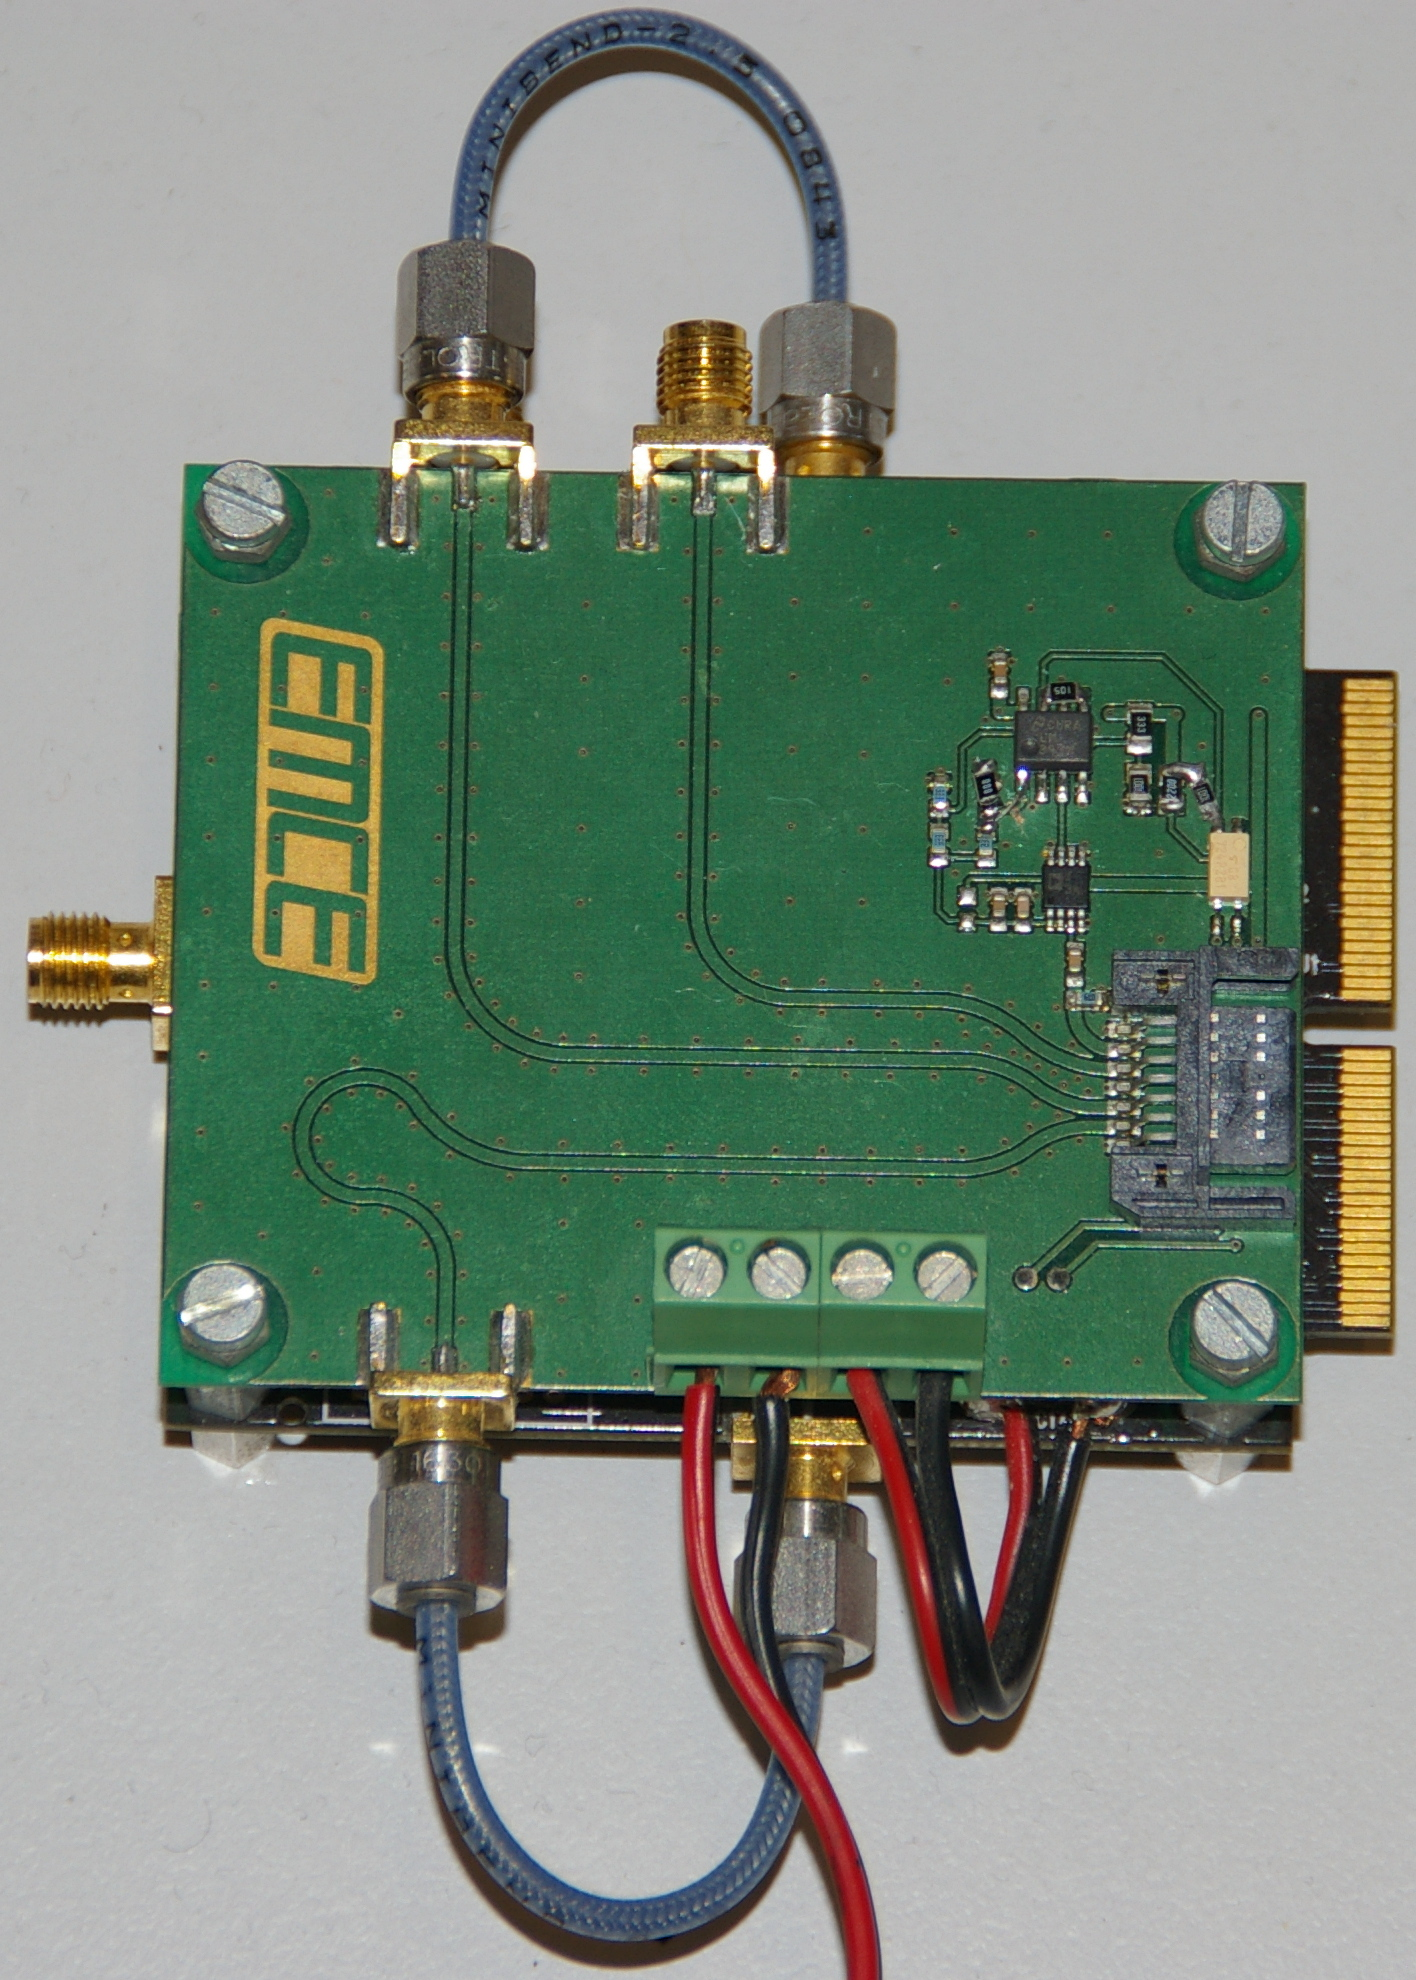
\includegraphics[width=\textwidth]{adc.jpg}};
            \begin{scope}[x={(image.south east)},y={(image.north west)},every node/.style={fill=white, fill opacity=0.8}]
                \draw (0,0.6) node[anchor=south west] {analog in};
                \draw (1,0) node[anchor=south east] {power supply};
                \draw (0.1,0.1) node[anchor=south west] {data+};
                \draw (0.2,1) node[anchor=north west] {data-};
                \draw (0.9,1) node[anchor=north east] (clk) {clock};
                \draw [-latex] (clk) -- (0.5,0.85);
                \draw (0.95,0.825) node[anchor=north east] {sync circuit};
                \draw (1,0.35) node[anchor=south east] {SATA};
            \end{scope}
        \end{tikzpicture}
        \caption{\gls{adc} adapter circuit board with disconnected clock line, atop the LTC2274 demo board}
        \label{fig:adc_adapter_circ}
    \end{subfigure}%
    ~
    \begin{subfigure}[c]{.45\linewidth}
        \centering
        \begin{tikzpicture}
            \node[inner sep=0pt] (image) at (0,0) {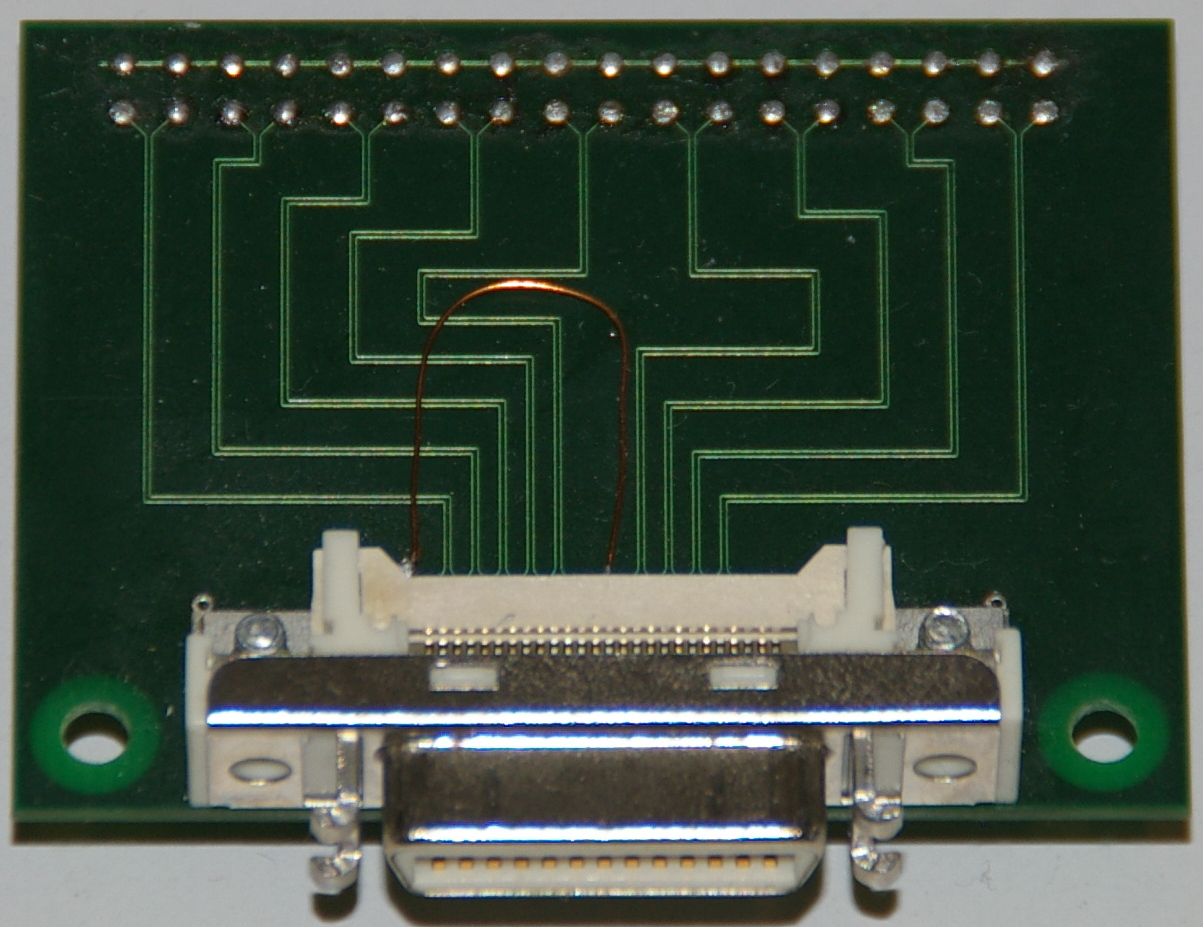
\includegraphics[width=\textwidth]{digital_iq.jpg}};
        \end{tikzpicture}
        \caption{Digital \gls{iq} adapter circuit board with S\_CLK fix}
        \label{fig:iq_adapter_circ}
    \end{subfigure}
    \caption{Photos of implemented adapter boards}
    \label{fig:adapters}
\end{figure}

% ===========================================================================

\chapter{\glsentryshort{fpga} Implementation}
\label{chap:fpga}

\begin{itemize}
    \item describe paper \cite{hashim_active_2008}
    \item improvements done
\end{itemize}

\section{Data Acquisition}
\label{sec:acquisition}
\begin{itemize}
    \item MSB \rightarrow LSB
    \item K28.5 D5.6/D16.2 (not JESD204B conform\cite{ltc2274}) \cite{jesd205B.01}
\end{itemize}
\section{Overlap Add}
\label{sec:overlap_add}
\section{SMBV Interface}
\label{sec:smbv_interface}

\begin{figure}[htb]
    \centering
    \tikzexternaldisable
    \begin{tikztimingtable}
        clk & c11{7c}c  \\
        ckm & c22{3.5c}c \\
        ckh & c77{c}c \\
        outdata\_long(0) & x2{14x}{}3{14d}7dd\\
        outdata\_long(1) & x3{14x}{}2{14d}7dd \\
        outdata\_long(2) & x{}4{14d}{}14d7dd \\
        outdata\_long(3) & x14x{}4{14d}{}7dd \\
        outdata\_short & [font=\scriptsize] x7d{(0)(6:3)}7d{(0)(2:0) (1)(6)}7d{(1)(5:2)}7d{(1)(1:0) (2)(6:5)}7d{(2)(4:1)}7d{(2)(0) (3)(6:4)}7d{(3)(3:0)}7d{(0)(6:3)}7d{(0)(2:0) (1)(6)}7d{(1)(5:2)}7d{(1)(1:0) (2)(6:5)}{}d \\
        out\_en & l49{l}28{h}h \\
    \end{tikztimingtable}
    \caption{LVDS Output generation timing. {\scriptsize (0)(2:0) (1)(6)} in \signal{outdata\_short} means {\ttfamily outdata\_long(0)(2 downto 0) \& outdata\_long(1)(6 downto 6)}.}
    \label{fig:trans}
\end{figure}

\section{Processor Interface}

% ===========================================================================

\chapter{Software Implementation}
\label{chap:software}
\section{Kernel Module}
\section{Network Server and Web-Interface}
\section{Matlab Driver}
\label{sec:matlab}


% ===========================================================================

\chapter{Verification of the Measurement System}
\label{chap:verification}

The implemented \gls{elp} design was tested with the setup in
\cref{fig:test_setup} at a center frequency $f_0$ of \SI{900}{\mega\hertz}. This test setup consists of the three parts
described in \cref{chap:measurement_system}. As mentioned in
\cref{sec:analog}, instead of a circulator, the directional coupler
\device{dir2} in combination with attenuator \device{att1} was used.
Furthermore, since during verification only waves generated inside
the specified bandwidth of \SI{20}{\mega\hertz} were used, the low-pass filter \device{lp2}
was used instead of a bandpass filter. A detailed list of used
instruments can be seen in \cref{sec:instruments}.

\begin{figure}[htb]
    \centering
    \resizebox{\linewidth}{!}{
    \begin{tikzpicture}
        \pgfdeclarelayer{foreground}
        \pgfsetlayers{background,main,foreground}
        \tikzpicturedependsonfile{rfsymbols.tex}
        \tikzstyle{every node}=[font=\footnotesize]
        \draw node[dut] (dut) {}
              node[dircoupler,right=2 of dut,label=below:dir1,label={[font=\tiny]above:\SI{-16}{\deci\bel}}] (dirvna) {}
              node[oscilloscope,above=of dirvna.A2,anchor=A1] (oszivna) {}
              node[dircouplera,right=of dirvna,label=below:dir2,label={[font=\tiny]above:\SI{-16}{\deci\bel}}] (dircirc) {}

              node[coordinate,above=2.5 of dircirc] (uppernode) {}

              node[attenuator,right=of dircirc,label=above:att1,label={[font=\tiny]below:\SI{10}{\deci\bel}}] (att) {}
              node[amplifier,right=of att,label=above:amp1] (amp) {}
              node[mixer,right=of amp,label=above:mix3] (upmix) {}
              node[lowpass,right=of upmix,label=above:lp1] (antialias) {}
              node[adc,right=of antialias,label=above:dac1] (dac) {}

              (uppernode -| upmix) node[mixer,label=below:mix1] (downmix) {}
              node[lowpass,right=of downmix,label=below:lp2,label={[font=\tiny]above:\SI{90}{\mega\hertz}}] (bp) {}
              node[adc,right=of bp,label=below:adc1] (adc) {}
              node[empty,right=of adc,label=below:buffer1] (inbuf) {}
              node[mixer,right=of inbuf] (shift) {}
              node[rotate=90,anchor=north] at (shift.east) {mix2}

              (dac -| inbuf) node[mixer,label=above:mul1] (mul) {}
              node[empty,right=of mul] (outbuf) {}
              node[rotate=90,anchor=north] at (outbuf.east) (buffer2) {buffer2}

              ($(shift)!.5!(outbuf)$) node[allpass,rotate=90] (H) {}
              node[rotate=90,anchor=north] at (H.south) {fir1}

              node[source,above=of downmix.center,scale=0.7] (downsource) {}
              node[rotate=90,anchor=south,font=\tiny] at (downsource.west) {$\SI{830}{\mega\hertz}$}
              node[rotate=90,anchor=north] at (downsource.east) {lo1}
              node[source,above=of adc.center,scale=0.7] (sample) {}
              node[rotate=90,anchor=south,font=\tiny] at (sample.west) {$\SI{100}{\mega\hertz}$}
              node[rotate=90,anchor=north] at (sample.east) {lo2}
              node[source,above=of shift.center,scale=0.7] (shiftsource) {}
              node[rotate=90,anchor=south,font=\tiny] at (shiftsource.west) {$\SI{30}{\mega\hertz}$}
              node[rotate=90,anchor=north] at (shiftsource.east) {lo3}
              node[source,below=of upmix.center,scale=0.7] (upsource) {}
              node[rotate=90,anchor=south,font=\tiny] at (upsource.west) {$\SI{900}{\mega\hertz}$}
              node[rotate=90,anchor=north] at (upsource.east) {lo4}
              node[below=of mul.center,fill=white] (gamma) {$\Gamma_{set}$};

        \draw ($(dut)!.5!(dirvna)$) node[coordinate] (plane) {};

        { [rounded corners=2pt]
            \draw (dut) -- (dirvna) -- (dircirc.A1);
            \draw [-latex] (dircirc.A2) |- (downmix);
            \draw (dirvna.A2) -- (oszivna.A1);
            \draw (dirvna.B2) |- ($(dirvna.B2)!.7!(oszivna.A2)$) node[coordinate] (oszimiddle) {} -| (oszivna.A2);
            \draw [-latex] (att) -- (dircirc.B1);
        }
        { [-latex]
            \draw (downsource) -- (downmix);
            \draw (sample) -- (adc);
            \draw [double] (shiftsource) -- (shift);
            \draw (gamma) -- (mul);
            \draw (upsource) -- (upmix);
        }
        { [latex-,dashed,every node/.style={font=\footnotesize}]
            \foreach \device in {downsource,sample} {
                \draw (\device) -- ++(0,1) node[anchor=south] {\SI{10}{\mega\hertz} ref};
            }
            \draw ([xshift=0.5cm]oszivna.north) -- ++(0,0.5) node[fill=white,anchor=south] {\SI{10}{\mega\hertz} ref};
        }
        { [start chain,every on chain/.style={join=by -latex}]
            \chainin (downmix);
            \chainin (bp);
            \chainin (adc);
            \chainin (inbuf);
            \chainin (shift);
            { [every on chain/.style={join=by {double,-latex}}]
                \chainin (H);
                \chainin (outbuf);
                \chainin (mul);
                \chainin (dac);
                \chainin (antialias);
                \chainin (upmix);
            }
            \chainin (amp);
            \chainin (att);
        }
        { [on background layer,every path/.style={dotted,decorate,decoration=random steps,segment length=2mm}]
            \draw ($(dirvna.B1)!.5!(dircirc.A1) + (0,5.5)$) -- ++(0,-8.5) node[coordinate] (leftsplit) {};
            \draw ($(adc.east)!.5!(mul.west) + (0,4)$) -- ++(0,-8.5) node[coordinate] (rightsplit) {};
        }

        \draw (leftsplit) node[anchor=base east] {One Port \gls{vna}}
              (leftsplit) node[anchor=base west] {Analog}
              (rightsplit) node[anchor=base west] {Digital}
              (rightsplit) node[anchor=base east] {Analog};

%        \draw [-latex] ($(dirvna.A2) + (-0.2,0.1)$) -- node[base left] {$b_1$} ($(oszivna.A1 |- oszimiddle) - (0.2,0.1)$);
%        \begin{pgfonlayer}{foreground}
%            \draw [-latex] ($(dirvna.B2) + (0.2,0.1)$) -- ($(oszimiddle -| dirvna.B2) + (0.2,-0.1)$);
%        \end{pgfonlayer}
%        \draw ($(oszimiddle -| dirvna.B2) + (0.2,-0.1)$) node[base right,fill=white] {$a_1$};

        \draw [dashed] ($(plane) + (0,5.5)$) node[anchor=south] {Load Reference Plane} -- ($(plane) - (0,3)$);

        \draw [latex-] ($(plane) + (0,1.5)$) -- ++(-0.5,0) node[anchor=east] {$Z_L$};

        \draw [-latex] ($(plane) + (0.25,-1.5)$) node[anchor=west] {$a_2$}-- ++(-0.5,0);
        \draw [latex-] ($(plane) + (0.25,-2)$) node[anchor=west] {$b_2$}-- ++(-0.5,0);
        \draw [latex-] ($(plane) + (0,-2.5)$) -- ++(-0.5,0) node[anchor=east] {$\Gamma_L$};
        \node [draw,fit=(amp) (dac) (upsource),rounded corners=4pt,inner xsep=6pt,inner ysep=14pt,label={above:Vector Signal Generator}] (sig) {};
        \draw [-latex,dashed] ([xshift=-2cm]sig.south) -- ++(0,-0.5) node[anchor=north] {\SI{10}{\mega\hertz} ref};
        \node [draw,fit=(gamma) (outbuf) (inbuf) (shiftsource) (buffer2),rounded corners=4pt,inner xsep=6pt,inner ysep=14pt,label={above:\gls{fpga}}] (fpga) {};

        {[densely dashdotdotted,latex-latex]
            \draw (fpga.east) -- ++(1,0) node [anchor=west] {\gls{pc}};
            \draw (sig.south) -- ++(0,-0.5) node [anchor=north] {\gls{pc}};
            \draw ([xshift=-0.5cm]oszivna.north) -- ++(0,1) node [anchor=south] {\gls{pc}};
        }
    \end{tikzpicture}
    }
    \caption{Measurement system verification test setup}
    \label{fig:test_setup}
\end{figure}

Since the overall setup consists of two independent systems, namely the one port
\gls{vna} and the reflection generation, those two were verified separately. The
one port \gls{vna} verification can be found in \cref{sec:vna_verify} and the
reflection generation, consisting of the analog part (see \cref{sec:analog}) and
the digital part (see \cref{sec:digital}), can be found in \cref{sec:reflection}.
During these measurements, a noticeable phase drift was observed, and therefore
an additional measurement was acquired, as seen in \cref{sec:drift}, to verify the origin
of this phase drift.

% ---------------------------------------------------------------------------

\section{One Port \glsentryshort{vna}}
\label{sec:vna_verify}

For the calibration and verification of the one port \gls{vna}, the modulator of
the vector signal generator was turned off. Stepping through the frequency range
was achieved by stepping the local oscillator \device{lo4} (see \cref{fig:test_setup}).
A ZV-Z132 (female) calibration kit from Rhode \& Schwarz was used for the calibration
setup in place of the \gls{dut}. Since the calibration is only valid for a single frequency, the full
calibration measurements were acquired for 21 $\Delta{}f$-aligned points in a
\SI{25}{\mega\hertz} range with a center frequency of \SI{900}{\mega\hertz}. This
was achieved by connecting the appropriate port of the calibration kit, and acquiring
$\Gamma_{L,f}$ for every frequency point. After the measurement, the different $\Gamma_{L,f}$ were linearly
interpolated at every $\Delta{}f$ bin. Afterwards the \glspl{sparam} of
the error box (see \cref{sec:vna}) were pre-calculated for every bin with the values
from the data sheet of the calibration kit\cite{zv-z132}.

For verification, a stub tuner from Maury Microwave was tuned to a specific position and
then measured with the one port \gls{vna} in this work. Measurements were acquired over
the whole \SI{25}{\mega\hertz} bandwidth at the calibrated points. Additional measurements
were acquired at an offset of $\frac{1}{2}\Delta{}f$, to be able to test the performance
of the chosen window function, and additionally between the calibrated points, to test the
performance of the interpolation. To be able to verify the measured $\Gamma_L$, measurements
were also acquired with a different \gls{vna}.

\begin{table}[htb]
    \centering
    \begin{tabular}{rrrr}
        \toprule
        \shortstack[r]{\textbf{frequency} \\ \si{\mega\hertz}} & \shortstack[r]{887.5\\(cal)} & \shortstack[r]{887.505\\($\frac{1}{2}\Delta{}f$)} & \shortstack[r]{888.095\\(between cal)} \\
        \midrule
        \shortstack[r]{\textbf{magnitude}\\ 1} & \num{581.0232e-003} & \num{581.0589e-003} & \num{582.3070e-003} \\
            standard error & \num{37.6e-006}     & \num{38.2e-006}     & \num{36.56e-006} \\
           $\Delta$Agilent \gls{vna} & \num{2.1e-003} & \num{2.1e-003} & \num{2.2e-003} \\
        \shortstack[r]{\textbf{angle}\\\si{\degree}}     & \num{-157.5029}     & \num{-157.4787}     & \num{-157.7972} \\
            standard error & \num{8.7e-003}      & \num{8.1e-003}      & \num{9.7e-003} \\
           $\Delta$Agilent \gls{vna} & \num{2.2} & \num{2.3} & \num{2.3} \\
        \bottomrule
    \end{tabular}
    \caption{Measured reflection coefficient with standard error and difference to Agilent \gls{vna}}
    \label{tab:vna}
\end{table}

No noticeable difference in standard error and difference to the results from the Agilent \gls{vna} between the three
different types of points, over the complete \SI{25}{\mega\hertz} range could be observed.
Therefore linear interpolation and the chosen window function are appropriate for this type of
measurement. Since there are only passive parts involved in the one port \gls{vna}, it should
also be possible to use less calibration points to achieve a faster calibration. The measurement
result of three exemplary points can be seen in \cref{tab:vna}.

The results are highly dependent on the used oscilloscope and calibration kit. The standard error
depends notably on the performance of the oscilloscope. Therefore these
results are only valid for the used oscilloscope in this work. Additionally care should be taken, to
always use a strong enough signal power, in order to achieve the best possible oscilloscope resolution.
The difference to the results from the Agilent \gls{vna} is mainly caused by the used calibration kit.

% ---------------------------------------------------------------------------

\section{Reflection Measurements}
\label{sec:reflection}

The reflection measurements were carried out with the test setup in \cref{fig:test_setup}
with an Agilent \gls{vna} as the \gls{dut}. The Agilent \gls{vna} was connected to the
\SI{10}{\mega\hertz} reference, in order to be able to generate the needed phase coherent
signals for the test setup. This allowed verifying the synthesized $\Gamma_L$, and
calibrating the \gls{fir} filter \device{fir1} more accurately, than using the built
in one port \gls{vna}.

The reflection generation consists of two tasks. First the iterative target algorithm
described in \cref{sec:matlab} is needed, to be able to synthesize specific $\Gamma_L$.
The performance of this algorithm can be seen in \cref{sec:iterative}. This
algorithm was then used for calibrating and verifying the filter \device{fir1}. Measurement
results with the calibrated filter can be seen in \cref{sec:filter}.

\subsection{Iterative target algorithm}
\label{sec:iterative}

\begin{figure}[htb]
    \begin{subfigure}[b]{.5\linewidth}
        \centering
        \begin{tikzpicture}[
            spy/.style={%
                draw,green,
                line width=0.5pt,
                circle,inner sep=0pt,
            },
            ]
            \def\spyviewersize{3cm}
            \def\spyonclipreduce{0.5pt}
            \def\spyfactorI{10}

            \def\pic#1#2{
                \begin{smithchart}[width=.9\linewidth,clip=false#1]
                    \addplot[blue,is smithchart cs] file {testdata/filter/1.0,0/trajectory10.data};
                    \addplot[purple,is smithchart cs,only marks,mark=x#2] file {testdata/filter/1.0,0/trajectory10.data};
                    \draw (cartesian cs:1,0) node[coordinate] (a) {}
                          (cartesian cs:-0.4,0.4) node[coordinate] (b) {};
                \end{smithchart}
            }
            \pic{}{}
            \coordinate (spy-on 1) at (a);
            \coordinate (spy-in 1) at (b);

            \node[spy,ultra thick,circular drop shadow,minimum size=\spyviewersize,fill=white,label={[inner sep=0pt,yshift=-5pt,fill=white,font=\footnotesize]below:\spyfactorI{}x magnification}] (spy-in node 1) at (spy-in 1) {};
            \begin{scope}
                \clip (spy-in 1) circle (0.5*\spyviewersize-\spyonclipreduce);
                \pgfmathsetmacro\sI{1/\spyfactorI}
                \begin{scope}[
                    shift={($\sI*(spy-in 1)-\sI*(spy-on 1)$)},
                    scale around={\spyfactorI:(spy-on 1)}
                ]
                \pic{,every axis plot post/.append style={line width=0.07pt},every axis/.append style={line width=0.07pt,grid style={line width=0.07pt}}}{,mark size=0.35pt}
                \end{scope}
            \end{scope}

        \end{tikzpicture}
        \caption{$\Gamma_{L,target} = 1$}
        \label{fig:find_target_good}
    \end{subfigure}%
    \begin{subfigure}[b]{.5\linewidth}
        \centering

        \begin{tikzpicture}[
            spy/.style={%
                draw,green,
                line width=0.5pt,
                circle,inner sep=0pt,
            },
            ]
            \def\spyviewersize{3cm}
            \def\spyonclipreduce{0.5pt}
            \def\spyfactorI{70}

            \def\pic#1#2{
                \begin{smithchart}[width=0.9\linewidth,clip=false#1]
                    \addplot[blue,is smithchart cs] file {testdata/filter/0.5,-45/trajectory6.data};
                    \addplot[purple,is smithchart cs,only marks,mark=x#2] file {testdata/filter/0.5,-45/trajectory6.data};
                    \draw (cartesian cs:0.35325,-0.35397) node[coordinate] (a) {}
                          (cartesian cs:-0.4,0.4) node[coordinate] (b) {};
                \end{smithchart}
            }
            \pic{}{}
            \coordinate (spy-on 1) at (a);
            \coordinate (spy-in 1) at (b);

            \node[spy,ultra thick,circular drop shadow,minimum size=\spyviewersize,fill=white,label={[inner sep=0pt,yshift=-5pt,fill=white,font=\footnotesize]below:\spyfactorI{}x magnification}] (spy-in node 1) at (spy-in 1) {};
            \begin{scope}
                \clip (spy-in 1) circle (0.5*\spyviewersize-\spyonclipreduce);
                \pgfmathsetmacro\sI{1/\spyfactorI}
                \begin{scope}[
                    shift={($\sI*(spy-in 1)-\sI*(spy-on 1)$)},
                    scale around={\spyfactorI:(spy-on 1)}
                ]
                    \pic{,every axis plot post/.append style={line width=0.01pt}}{,mark size=0.05pt}
                \end{scope}
            \end{scope}
        \end{tikzpicture}
        \caption{$\Gamma_{L,target} = 0.5 \angle \SI{-45}{\degree}$}
        \label{fig:find_target_bad}
    \end{subfigure}
    \caption{Exemplary trajectories of the target algorithm}
    \label{fig:find_target}
\end{figure}

The target algorithm as described in \cref{sec:matlab}, is able to find the
correct $\Gamma_{L,set}$ with a given $\Gamma_{L,start}$ in order to synthesize
a given $\Gamma_L$. All the following measurements used 20000 samples as
sample period $n$ (see \cref{sec:acquisition}), an $L$ of 2000 and an \gls{fft} width $n_{fft}$
of 4096 (see \cref{fig:overlap_add}). The filter \device{fir1} was preloaded with the
impulse response of a low pass filter with a cut off frequency of \SI{25}{\mega\hertz} to
filter out the aliases (see \cref{sec:digital}). For the duration of these measurements,
the \gls{fpga} implementation was switched to automatic mode (see \cref{chap:fpga}). The digital reflection generation introduces
a very high latency on the order of about \SI{1}{\milli\second} with this settings.
Therefore a wait time of \SI{100}{\milli\second} was used for the iterative algorithm
(see \cref{sec:matlab}). This allows the system to settle on a $\Gamma_L$ before continuing
with the algorithm. If the wait time is too short, this algorithm can start to
cause oscillations and the completion time of the algorithm actually increases. Whereas
a long wait time increases the completion time.

\begin{figure}[htb]
    \centering
    \begin{tikzpicture}
        \begin{axis}[
                ybar interval,
                ylabel={percentage of invocations},
                xlabel={number of iterations},
                x filter/.expression={x-1}, % remove the start point
                ymin = 0
            ]
            \addplot[blue,fill=blue!10,hist={bins=7,data min=3,data max=10,density=true}] table[y index=0] {testdata/trajectories/performance.data};
        \end{axis}
    \end{tikzpicture}
    \caption{Histogram of algorithm iterations needed to find a specific $\Gamma_L$}
    \label{fig:iteration_hist}
\end{figure}

Two descriptive example trajectories can be seen in \cref{fig:find_target}. In
\cref{fig:find_target_good} the algorithm terminated just after three steps,
whereas in \cref{fig:find_target_bad} the worst observed case can be seen. The
trajectory in \cref{fig:find_target_bad} oscillates around the target before
reaching it. This is caused either by a too stringent termination condition, or
by a bad resolution of the \gls{vna} or the digital part of this system, in the
target range.

Depending on the start point $\Gamma_{L,start}$ and the target $\Gamma_{L}$
the performance of the algorithm varied. An overall histogram of 108 different
invocations with different $\Gamma_{L,start}$, different $\Gamma_{L,target}$ and
at different frequencies can be seen in \cref{fig:iteration_hist}. The trajectory
in \cref{fig:find_target_bad} is the only one in bin 8.

As can be seen in \cref{fig:find_target,fig:iteration_hist} the algorithm is capable
of reaching a specified reflection coefficient $\Gamma_{L,target}$ within a reasonable
amount of time. Keeping the limitations above in mind the algorithm could be further
accelerated by adjusting the termination condition and the settling time.

\subsection{Filter performance}
\label{sec:filter}

For verification, the filter \device{fir1} in \cref{fig:test_setup} was calibrated
by measuring the needed $\Gamma_{L,set}$ to achieve a specific $\Gamma_L$ over a
baseband range from \SI{-13}{\mega\hertz} to \SI{13}{\mega\hertz} at a \gls{rf} of
\SI{900}{\mega\hertz} (see \cref{sec:matlab}). All following
measurements used the same settings as described in \cref{sec:iterative}, a sample period $n$ of 20000,
$L$ of 2000 and an \gls{fft} width $n_{fft}$ of 4096 (see also \cref{fig:overlap_add}).
Before calibration the filter \device{fir1} was preloaded with a low pass filter, with
a cut off frequency of \SI{25}{\mega\hertz} to filter out the aliases (see
\cref{sec:digital}). For the duration of the measurements, the \gls{fpga} implementation
was switched to automatic mode (see \cref{chap:fpga}). Filter calibration was then carried out at the following $\Gamma_L$
values: $1$, $-1$, $0.5\angle\SI{135}{\degree}$ and $0.5\angle\SI{-45}{\degree}$. Additional
verification measurements were carried out with the mean of the acquired measurements
at $1$ and $-1$, as well as the mean of the measurements at $0.5\angle\SI{135}{\degree}$
and $0.5\angle\SI{-45}{\degree}$. For the following verification measurements, the respective
calibration measurement was added to the filter \device{fir1} by linearly interpolating
the measured $\Gamma_{L,set}$ at every $\Delta{}f$-bin of the filter and then multiplying
these values with the impulse response of the above mentioned alias filter.

The verification measurements were acquired with the Agilent \gls{vna} at frequencies
ranging from \SI{895}{\mega\hertz} to \SI{905}{\mega\hertz} in \SI{1}{\mega\hertz} steps
with a settling time of \SI{0.5}{\second} for every frequency point. To be able to verify
the performance across the whole range, measurements were acquired over the possible
$\Gamma_{L,set}$ range by stepping through an 11 by 11 grid. These measurements were
acquired with the different filter calibrations mentioned above.

The results, which can be seen in \cref{fig:calibrated_filter}, contain every acquired
trajectory in blue and the calibration point in red. Since only the filter \device{fir1}
was calibrated, but neither the target algorithm, nor an error model was used for the
$\Gamma_{L,set}$ values, the overall grid is slightly distorted. As can be seen in these
smith charts, the trajectories spread out at points far away from the calibration points.
As expected, the filter calibrations with the mean values achieve better trajectories
between the calibration points. Since the trajectories around the calibration points
show the best performance, it is advisable to use calibration points near the expected
target $\Gamma_L$ and avoid calibration points at $\abs{\Gamma_L} = 1$. Noticeable
trajectory spreading near the calibration points is caused by the limited numerical
precision of the filter implementation of \device{fir1} (see \cref{sec:overlap_add}).

\begin{figure}[htbp]
    \centering
    \begin{subfigure}[b]{.45\linewidth}
        \centering
        \begin{tikzpicture}
            \begin{smithchart}[width=.9\linewidth,clip=false]
                \foreach \i in {1,...,11}{
                    \foreach \j in {1,...,11}{
                        \addplot[blue,is smithchart cs] file {testdata/filter/1.0,180/\i,\j.data};
                    }
                }
                \addplot[red,is smithchart cs,mark=*,only marks] coordinates {(-1,0)};
            \end{smithchart}
        \end{tikzpicture}
        \caption{$-1$}
    \end{subfigure}%
    \begin{subfigure}[b]{.45\linewidth}
        \centering
        \begin{tikzpicture}
            \begin{smithchart}[width=.9\linewidth,clip=false]
                \foreach \i in {1,...,11}{
                    \foreach \j in {1,...,11}{
                        \addplot[blue,is smithchart cs] file {testdata/filter/0.5,135/\i,\j.data};
                    }
                }
                \addplot[red,is smithchart cs,mark=*,only marks] coordinates {(-0.3536,0.3536)};
            \end{smithchart}
        \end{tikzpicture}
        \caption{$0.5 \angle \SI{135}{\degree}$}
    \end{subfigure}\\
    \begin{subfigure}[b]{.45\linewidth}
        \centering
        \begin{tikzpicture}
            \begin{smithchart}[width=.9\linewidth,clip=false]
                \foreach \i in {1,...,11}{
                    \foreach \j in {1,...,11}{
                        \addplot[blue,is smithchart cs] file {testdata/filter/1.0,0/\i,\j.data};
                    }
                }
                \addplot[red,is smithchart cs,mark=*,only marks] coordinates {(+1,0)};
            \end{smithchart}
        \end{tikzpicture}
        \caption{$1$}
    \end{subfigure}%
    \begin{subfigure}[b]{.45\linewidth}
        \centering
        \begin{tikzpicture}
            \begin{smithchart}[width=.9\linewidth,clip=false]
                \foreach \i in {1,...,11}{
                    \foreach \j in {1,...,11}{
                        \addplot[blue,is smithchart cs] file {testdata/filter/0.5,-45/\i,\j.data};
                    }
                }
                \addplot[red,is smithchart cs,mark=*,only marks] coordinates {(0.3536,-0.3536)};
            \end{smithchart}
        \end{tikzpicture}
        \caption{$0.5 \angle \SI{-45}{\degree}$}
    \end{subfigure}\\
    \begin{subfigure}[b]{.45\linewidth}
        \centering
        \begin{tikzpicture}
            \begin{smithchart}[width=.9\linewidth,clip=false]
                \foreach \i in {1,...,11}{
                    \foreach \j in {1,...,11}{
                        \addplot[blue,is smithchart cs] file {testdata/filter/mean1/\i,\j.data};
                    }
                }
                \addplot[red,is smithchart cs,mark=*,only marks] coordinates {(-1,0) (+1,0)};
            \end{smithchart}
        \end{tikzpicture}
        \caption{$mean(-1,1)$}
    \end{subfigure}%
    \begin{subfigure}[b]{.45\linewidth}
        \centering
        \begin{tikzpicture}
            \begin{smithchart}[width=.9\linewidth,clip=false]
                \foreach \i in {1,...,11}{
                    \foreach \j in {1,...,11}{
                        \addplot[blue,is smithchart cs] file {testdata/filter/mean2/\i,\j.data};
                    }
                }
                \addplot[red,is smithchart cs,mark=*,only marks] coordinates {(0.3536,-0.3536) (-0.3536,0.3536)};
            \end{smithchart}
        \end{tikzpicture}
        \caption{$mean(0.5 \angle \SI{135}{\degree}, 0.5 \angle \SI{-45}{\degree})$}
    \end{subfigure}
    \caption{Reflection measurements with calibrated filter}
    \label{fig:calibrated_filter}
\end{figure}

% ---------------------------------------------------------------------------

\section{Phase Drift}
\label{sec:drift}

During the measurements, phase drift could be noticed. In order to examine the
cause of these phase drifts, a test measurement was acquired, to be able
to observe the extent of the phase drift. For this measurement the test setup
in \cref{fig:test_setup} with the Agilent \gls{vna} (see \cref{sec:instruments})
as \gls{dut} was used. This \gls{vna} was also connected to the
\SI{10}{\mega\hertz} reference, in order to generate phase coherent signals. The
\gls{fpga} implementation was set to 20000 samples as the sample period $n$, an $L$
of 2000 and a \gls{fft} width $n_{fft}$ of 4096 (see \cref{fig:overlap_add}).
According to \cref{sec:digital} \device{fir1} needs at least a low pass filter to
filter out the aliases. Therefore it was preloaded with the impulse response of a low pass filter
with a cut off frequency of \SI{25}{\mega\hertz}. For the duration of the measurements,
the \gls{fpga} implementation was switched to automatic mode (see \cref{chap:fpga}). After
those preparations the system was set to a reflection coefficient $\Gamma_L = 1$ with
the target algorithm. Measurements were acquired every \SI{10}{\second} for a duration
of \SI{1000}{\minute}. The results of those phase drift measurements can be seen in
\cref{fig:phase_single}, which shows the angle of $\Gamma_L$ over time. Since the magnitude did not change noticeably during those measurements
it was left out of the plot.

\begin{figure}[htb]
    \centering
    \begin{tikzpicture}
        \begin{axis}[
                ylabel={angle},
                y unit={\degree},
                xlabel={time},
                x unit={\minute}, %change xbase
                width=\linewidth,
                x filter/.expression={x/60},
                xmin=0,
                xmax=1000,
                height=7cm
            ]
            \addplot[blue] table {testdata/phase/single.data};
        \end{axis}
    \end{tikzpicture}
    \caption{Phase drift of $\Gamma_L$}
    \label{fig:phase_single}
\end{figure}

These results indicate, that the phase drift is not caused by the filter implementation of
\device{fir1}, which would also cause changes of magnitude. Because of that, the test
setup in \cref{fig:setup_phase_single} was devised to measure the phase drift of all the
used local oscillators in the setup. This setup consists of oscilloscopes to measure
the different signals generated by the signal generators. Since the frequencies
of the generators were \SI{830}{\mega\hertz}, \SI{100}{\mega\hertz} and \SI{900}{\mega\hertz},
the additional function generator \device{trigger} (see \cref{fig:setup_phase_single}) was needed to
generate the greatest common divisor of those frequencies, which is \SI{10}{\mega\hertz}.
It was not possible to generate a good enough trigger signal with this function generator, that
allowed reliably measuring the phase of the different signals. Therefore this signal was also recorded.
To be able to measure all the signals, a second oscilloscope had to be used. Since triggering
the second oscilloscope with the first one resulted in a worse performance, than feeding both
oscilloscopes with the same trigger, a chained setup was not used. After the measurement, the
different signals were corrected by the phase offset of the trigger signal, to achieve a phase
offset of the trigger signal of zero. Therefore the results are the same as if the oscilloscopes would
have triggered perfectly. For a list of the used instruments see \cref{sec:instruments}.
Like with the measurement of the whole test setup, a phase offset was acquired every \SI{10}{\second}
for \SI{1000}{\minute}.

\begin{figure}[htb]
    \centering
    \begin{tikzpicture}
        \tikzpicturedependsonfile{rfsymbols.tex}
        \tikzstyle{every node}=[font=\footnotesize]
        \draw node[vna] (vna) {}
              node[source,right=of vna,scale=0.7] (downsource) {}
              node[rotate=90,anchor=south,font=\tiny] at (downsource.west) {$\SI{830}{\mega\hertz}$}
              node[rotate=90,anchor=north] at (downsource.east) {lo1}
              node[source,right=of downsource,scale=0.7] (sample) {}
              node[rotate=90,anchor=south,font=\tiny] at (sample.west) {$\SI{100}{\mega\hertz}$}
              node[rotate=90,anchor=north] at (sample.east) {lo2}
              node[source,right=of sample,scale=0.7] (trigger) {}
              node[rotate=90,anchor=south,font=\tiny] at (trigger.west) {$\SI{10}{\mega\hertz}$}
              node[rotate=90,anchor=north] at (trigger.east) {trigger}
              node[source,right=of trigger,scale=0.7] (upsource) {}
              node[rotate=90,anchor=south,font=\tiny] at (upsource.west) {$\SI{900}{\mega\hertz}$}
              node[rotate=90,anchor=north] at (upsource.east) {lo4}

              node[oscilloscope,above=2 of downsource] (oszi1) {}
              node[oscilloscope,right=of oszi1] (oszi2) {};

        {[densely dashdotdotted,latex-latex]
            \draw ([xshift=-0.5cm]oszi1.north) -- ++(0,1) node [anchor=south] {\gls{pc}};
            \draw ([xshift=-0.5cm]oszi2.north) -- ++(0,1) node [anchor=south] {\gls{pc}};
        }
        {[latex-,dashed,every node/.style={font=\footnotesize},rounded corners=2pt]
            \draw [latex reversed-,shorten <=1pt] (upsource) -- ++(0,-1) node[coordinate] (lower) {} -- ++(1,0) node[coordinate] (lowerright) {};
            \draw ([xshift=0.5cm]oszi2.north) -- ++(0,0.5) node[coordinate] (upper) {} -| (lowerright);
            \draw ([xshift=0.5cm]oszi1.north) |- (upper);
            \draw (trigger) |- (lower);
            \draw (sample) |- (trigger |- lower);
            \draw (downsource) |- (sample |- lower) node[anchor=north] {\SI{10}{\mega\hertz} ref};
            \draw (vna) |- (downsource |- lower);
        }
        {[rounded corners=2pt]
            \draw (vna) -- ++(0,1) -| (oszi1.A1);
            \draw (downsource) -- ++(0,1) -| (oszi1.A2);
            \draw (sample) -- ++(0,1.2) -| (oszi1.A3);
            \draw (trigger) -- ++(0,1.4) -| (oszi1.A4);
            \draw (trigger) -- ++(0,1.6) -| (oszi2.A1);
            \draw (upsource) -- ++(0,1.8) -| (oszi2.A2);
        }
    \end{tikzpicture}
    \caption{Phase drift measurement setup}
    \label{fig:setup_phase_single}
\end{figure}

The measurement results, which can be seen in \cref{fig:phase_overall}, show a
trend of the phase drift of every instrument. The phase drift in those instruments is likely
caused in part by phase drift of the oscillators in the instruments. Another part is caused by
the low reference frequency of \SI{10}{\mega\hertz}. During a single period of the reference
signal, a lot of periods need to be generated by the instruments, allowing only far apart
synchronisation points. A further component is temperature drift, since the room temperature
of the laboratory was not held constant. For these reasons the measurement results in
\cref{fig:phase_overall} are only exemplary and don't show the real phase drift, since
the trigger source \device{trigger} and the two oscilloscopes also experience phase drift.

\begin{figure}[htb]
    \centering
    \begin{tikzpicture}
        \pgfplotstableread{testdata/phase/all.data}\phaseall
        \begin{axis}[
                ylabel={angle},
                y unit={\degree},
                xlabel={time},
                x unit={\minute},
                x filter/.expression={x/60},
                xmin=0,
                xmax=1000,
                width=\linewidth,
                height=7cm,
                legend style={at={(0.5,1.01)},anchor=south},
                legend columns=4
            ]
            \addplot[blue] table {\phaseall};
            \addlegendentry{\glsentryshort{vna}}
            \addplot[green] table[x index=0,y index=2] {\phaseall};
            \addlegendentry{\device{lo1}}
            \addplot[red] table[y index=3] {\phaseall};
            \addlegendentry{\device{lo2}}
            \addplot[black] table[y index=4] {\phaseall};
            \addlegendentry{\device{lo4}}
        \end{axis}
    \end{tikzpicture}
    \caption{Phase drift of signal generators}
    \label{fig:phase_overall}
\end{figure}

The above mentioned phase drift needs to be kept in mind during measurements. This
drift causes additional phase errors in the resulting $\Gamma_L$ and, depending on
the accuracy needed of the measurements, limits the valid time of the calibration of
the different parts of the measurement setup.

% ===========================================================================

\chapter{Conclusions and Outlook}

\begin{appendix}
    \chapter{Hardware Reference}
    \section{Used Instruments}
    \label{sec:instruments}
    \section{Physical Overview}
    \section{Memory Map \& Register Assignment}
    \chapter{Software Reference}
    \section{Kernel Module Usage}
    \section{Protocols}
    \section{Matlab Classes}
    \section{Usage Examples}
    \chapter{Build Instructions}
    \section{Hardware}
    \section{Software}

    \printglossary[type=\acronymtype]

    \listoffigures

    \bibliographystyle{IEEEtran}
    \bibliography{main}

\begin{otherlanguage}{ngerman}
    \chapter*{Code of Conduct}
    Hiermit erkl\"are ich, dass die vorliegende Arbeit ohne unzul\"assige Hilfe Dritter und ohne Benutzung
    anderer als der angegebenen Hilfsmittel angefertigt wurde. Die aus anderen Quellen oder indirekt
    \"ubernommenen Daten und Konzepte sind unter Angabe der Quelle gekennzeichnet.
    Die Arbeit wurde bisher weder im In- noch im Ausland in gleicher oder in \"ahnlicher Form in anderen
    Pr\"ufungsverfahren vorgelegt.

    \par\noindent\makebox[7cm]{\hrulefill}      \hfill\makebox[5cm]{\hrulefill}%
    \par\noindent\makebox[7cm][l]{Unterschrift} \hfill\makebox[5cm][l]{Datum}%
\end{otherlanguage}

    \end{appendix}
\end{document}

